\documentclass[]{book}
\usepackage{lmodern}
\usepackage{amssymb,amsmath}
\usepackage{ifxetex,ifluatex}
\usepackage{fixltx2e} % provides \textsubscript
\ifnum 0\ifxetex 1\fi\ifluatex 1\fi=0 % if pdftex
  \usepackage[T1]{fontenc}
  \usepackage[utf8]{inputenc}
\else % if luatex or xelatex
  \ifxetex
    \usepackage{mathspec}
  \else
    \usepackage{fontspec}
  \fi
  \defaultfontfeatures{Ligatures=TeX,Scale=MatchLowercase}
\fi
% use upquote if available, for straight quotes in verbatim environments
\IfFileExists{upquote.sty}{\usepackage{upquote}}{}
% use microtype if available
\IfFileExists{microtype.sty}{%
\usepackage{microtype}
\UseMicrotypeSet[protrusion]{basicmath} % disable protrusion for tt fonts
}{}
\usepackage[margin=1in]{geometry}
\usepackage{hyperref}
\hypersetup{unicode=true,
            pdftitle={Experimentum: Web-based Software for Psychology Studies},
            pdfauthor={Rebecca J. Lai, Rifah Abdullah, Gaby Mahrholz, Lisa DeBruine},
            pdfborder={0 0 0},
            breaklinks=true}
\urlstyle{same}  % don't use monospace font for urls
\usepackage{color}
\usepackage{fancyvrb}
\newcommand{\VerbBar}{|}
\newcommand{\VERB}{\Verb[commandchars=\\\{\}]}
\DefineVerbatimEnvironment{Highlighting}{Verbatim}{commandchars=\\\{\}}
% Add ',fontsize=\small' for more characters per line
\usepackage{framed}
\definecolor{shadecolor}{RGB}{248,248,248}
\newenvironment{Shaded}{\begin{snugshade}}{\end{snugshade}}
\newcommand{\KeywordTok}[1]{\textcolor[rgb]{0.13,0.29,0.53}{\textbf{#1}}}
\newcommand{\DataTypeTok}[1]{\textcolor[rgb]{0.13,0.29,0.53}{#1}}
\newcommand{\DecValTok}[1]{\textcolor[rgb]{0.00,0.00,0.81}{#1}}
\newcommand{\BaseNTok}[1]{\textcolor[rgb]{0.00,0.00,0.81}{#1}}
\newcommand{\FloatTok}[1]{\textcolor[rgb]{0.00,0.00,0.81}{#1}}
\newcommand{\ConstantTok}[1]{\textcolor[rgb]{0.00,0.00,0.00}{#1}}
\newcommand{\CharTok}[1]{\textcolor[rgb]{0.31,0.60,0.02}{#1}}
\newcommand{\SpecialCharTok}[1]{\textcolor[rgb]{0.00,0.00,0.00}{#1}}
\newcommand{\StringTok}[1]{\textcolor[rgb]{0.31,0.60,0.02}{#1}}
\newcommand{\VerbatimStringTok}[1]{\textcolor[rgb]{0.31,0.60,0.02}{#1}}
\newcommand{\SpecialStringTok}[1]{\textcolor[rgb]{0.31,0.60,0.02}{#1}}
\newcommand{\ImportTok}[1]{#1}
\newcommand{\CommentTok}[1]{\textcolor[rgb]{0.56,0.35,0.01}{\textit{#1}}}
\newcommand{\DocumentationTok}[1]{\textcolor[rgb]{0.56,0.35,0.01}{\textbf{\textit{#1}}}}
\newcommand{\AnnotationTok}[1]{\textcolor[rgb]{0.56,0.35,0.01}{\textbf{\textit{#1}}}}
\newcommand{\CommentVarTok}[1]{\textcolor[rgb]{0.56,0.35,0.01}{\textbf{\textit{#1}}}}
\newcommand{\OtherTok}[1]{\textcolor[rgb]{0.56,0.35,0.01}{#1}}
\newcommand{\FunctionTok}[1]{\textcolor[rgb]{0.00,0.00,0.00}{#1}}
\newcommand{\VariableTok}[1]{\textcolor[rgb]{0.00,0.00,0.00}{#1}}
\newcommand{\ControlFlowTok}[1]{\textcolor[rgb]{0.13,0.29,0.53}{\textbf{#1}}}
\newcommand{\OperatorTok}[1]{\textcolor[rgb]{0.81,0.36,0.00}{\textbf{#1}}}
\newcommand{\BuiltInTok}[1]{#1}
\newcommand{\ExtensionTok}[1]{#1}
\newcommand{\PreprocessorTok}[1]{\textcolor[rgb]{0.56,0.35,0.01}{\textit{#1}}}
\newcommand{\AttributeTok}[1]{\textcolor[rgb]{0.77,0.63,0.00}{#1}}
\newcommand{\RegionMarkerTok}[1]{#1}
\newcommand{\InformationTok}[1]{\textcolor[rgb]{0.56,0.35,0.01}{\textbf{\textit{#1}}}}
\newcommand{\WarningTok}[1]{\textcolor[rgb]{0.56,0.35,0.01}{\textbf{\textit{#1}}}}
\newcommand{\AlertTok}[1]{\textcolor[rgb]{0.94,0.16,0.16}{#1}}
\newcommand{\ErrorTok}[1]{\textcolor[rgb]{0.64,0.00,0.00}{\textbf{#1}}}
\newcommand{\NormalTok}[1]{#1}
\usepackage{longtable,booktabs}
\usepackage{graphicx,grffile}
\makeatletter
\def\maxwidth{\ifdim\Gin@nat@width>\linewidth\linewidth\else\Gin@nat@width\fi}
\def\maxheight{\ifdim\Gin@nat@height>\textheight\textheight\else\Gin@nat@height\fi}
\makeatother
% Scale images if necessary, so that they will not overflow the page
% margins by default, and it is still possible to overwrite the defaults
% using explicit options in \includegraphics[width, height, ...]{}
\setkeys{Gin}{width=\maxwidth,height=\maxheight,keepaspectratio}
\IfFileExists{parskip.sty}{%
\usepackage{parskip}
}{% else
\setlength{\parindent}{0pt}
\setlength{\parskip}{6pt plus 2pt minus 1pt}
}
\setlength{\emergencystretch}{3em}  % prevent overfull lines
\providecommand{\tightlist}{%
  \setlength{\itemsep}{0pt}\setlength{\parskip}{0pt}}
\setcounter{secnumdepth}{5}
% Redefines (sub)paragraphs to behave more like sections
\ifx\paragraph\undefined\else
\let\oldparagraph\paragraph
\renewcommand{\paragraph}[1]{\oldparagraph{#1}\mbox{}}
\fi
\ifx\subparagraph\undefined\else
\let\oldsubparagraph\subparagraph
\renewcommand{\subparagraph}[1]{\oldsubparagraph{#1}\mbox{}}
\fi

%%% Use protect on footnotes to avoid problems with footnotes in titles
\let\rmarkdownfootnote\footnote%
\def\footnote{\protect\rmarkdownfootnote}

%%% Change title format to be more compact
\usepackage{titling}

% Create subtitle command for use in maketitle
\providecommand{\subtitle}[1]{
  \posttitle{
    \begin{center}\large#1\end{center}
    }
}

\setlength{\droptitle}{-2em}

  \title{Experimentum: Web-based Software for Psychology Studies}
    \pretitle{\vspace{\droptitle}\centering\huge}
  \posttitle{\par}
    \author{Rebecca J. Lai, Rifah Abdullah, Gaby Mahrholz, Lisa DeBruine}
    \preauthor{\centering\large\emph}
  \postauthor{\par}
      \predate{\centering\large\emph}
  \postdate{\par}
    \date{2020-04-06}


\begin{document}
\maketitle

{
\setcounter{tocdepth}{1}
\tableofcontents
}
\chapter*{About Experimentum}\label{about-experimentum}
\addcontentsline{toc}{chapter}{About Experimentum}

\subsection*{Getting Support}\label{support}
\addcontentsline{toc}{subsection}{Getting Support}

\subsubsection*{For Experimentum @ University of Glasgow
Users}\label{for-experimentum-university-of-glasgow-users}
\addcontentsline{toc}{subsubsection}{For Experimentum @ University of
Glasgow Users}

Currently there are two active admins available to provide support,
these are \href{mailto:rebecca.lai@glasgow.ac.uk}{Rebecca Lai} and
\href{mailto:lisa.debruine@glasgow.ac.uk}{Professor Lisa DeBruine}.

Admins play a double role. In addition to helping you with Experimentum
we are active researchers and teaching staff with additional jobs to do
elsewhere. Our inboxes are often full, and emails will often go unread.

As a result of this, all students and staff who are experiencing
technical issues should use the Slack workspace
\href{https://experimentum-web.slack.com/}{``Experimentum-web''} to get
support. Additionally, we are using the queries on the slack workspace
to best update the user documentation, so it is important to keep all
correspondence in one neat location.

\begin{rainbow}
You should never post data on this workspace, either in data file or
screenshot form, as this would be a violation of the GDPR. All such
files will be removed and your supervisor will be informed.

If you need to share your data please use one of the university approved
services available to you, such as OneDrive or OwnCloud.
\end{rainbow}

\hypertarget{lost_password}{\subsubsection*{Lost
Passwords}\label{lost_password}}
\addcontentsline{toc}{subsubsection}{Lost Passwords}

You can now reset your password without having to consult a system
admin. You can do this by going to the login page, supplying your user
ID or email address in the ``Username'' box and pressing the ``Reset
Password'' button, as shown below:

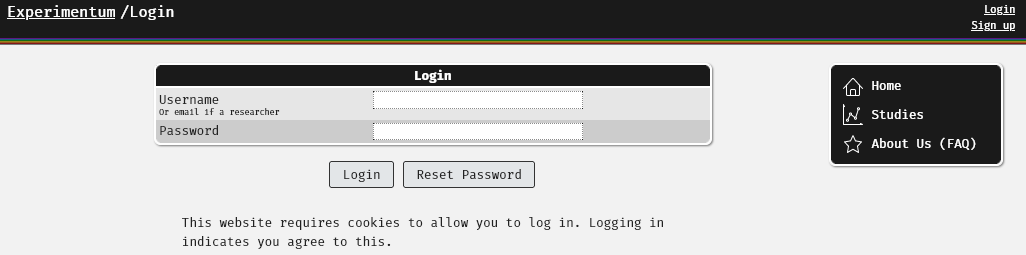
\includegraphics{images/screenshots/login.png}

\begin{warning}
If you have reset your password you will be supplied with a randomly
generated one to your \emph{registered email address}.

You should change this as soon as possible, if not immediately.
\end{warning}

If you do not have access to the registered email inbox please speak to
your supervisor or the admins who may be able to reset your password for
you on production of valid ID.

\subsubsection*{Changing Your Password}\label{changing-your-password}
\addcontentsline{toc}{subsubsection}{Changing Your Password}

You can change your password by signing in, navigating to ``My Account''
from the menu on the right of the page and clicking the link ``change
your password'' under ``Username'':

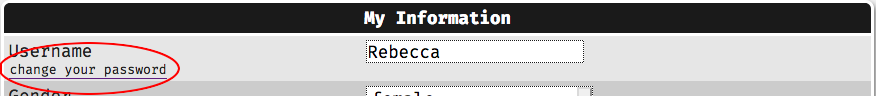
\includegraphics{images/screenshots/change_password.png}

\subsubsection*{Tutorial Sessions}\label{tutorial-sessions}
\addcontentsline{toc}{subsubsection}{Tutorial Sessions}

During times of particularly heavy use through the academic year we may
schedule specific help sessions to deal with common issues and to help
you fix specific problems that you might have. These will be advertised
on the Slack workspace and on appropriate Moodle pages.

If you are experiencing an issue that is particularly difficult to fix
remotely, you can make an appointment with Rebecca via private message
on the \href{https://experimentum-web.slack.com/}{``Experimentum-web''}
workspace. However, you should have made attempts to solve the issue
remotely first as time available for these appointments is extremely
limited.

If you require assistance to navigate this document or create your study
due to disability please contact your supervisor who may refer you to
the admins.

\subsubsection*{For Other Users @ Other
Institutions}\label{for-other-users-other-institutions}
\addcontentsline{toc}{subsubsection}{For Other Users @ Other
Institutions}

If you download and use the code for this platform you should establish
clear guidelines outlining the role of the admins and methods of support
in accordance with any relevant regulations.

Staff from the University of Glasgow will not provide support for users
of other systems based upon this code. Our Slack workspace is for
internal use only.

\begin{rainbow}
Experimentum is an evolving platform.

If you find an issue with the Experimentum codebase, you can file an
issue \href{https://github.com/debruine/experimentum/issues}{here}.

If you find an issue with the codebase for this manual you can file an
issue \href{https://github.com/RebeccaJLai/exp_manual/issues}{here}.
\end{rainbow}

\section*{Privacy Notices}\label{privacy-notices}
\addcontentsline{toc}{section}{Privacy Notices}

\subsection*{Cookies}\label{cookies}
\addcontentsline{toc}{subsection}{Cookies}

Cookies are used for Experimentum to allow us to track user sessions,
which allows participants to navigate between pages during a session
without having to log in to every page. In the case of anonymous logins,
the session is tracked to maintain the same identity across multiple
elements of the same study.

Cookies are not tracked beyond a single session, for either registered
or anonymous participants. By closing the browser the current session is
ended and cookies tracking the session are discarded.

Cookies are not used in any other way by us, and the information is not
retained or shared with any other organisations.

\subsection*{Data Management}\label{data-management}
\addcontentsline{toc}{subsection}{Data Management}

Your study's data is your responsibility. Please ensure that it is
protected and used appropriately. University of Glasgow guidelines with
regard to data protection are available to view
\href{https://www.gla.ac.uk/myglasgow/dpfoioffice/}{here} and more
general data management guidelines
\href{https://www.gla.ac.uk/myglasgow/datamanagement/rdmatglasgow/}{here}.

Experimentum saves your data to the University of Glasgow School of
Psychology secure servers, which are on-site in Hillhead Street. Data
will be output in Comma Separated Value (.csv) files in ``tidy'' format
and is available for download from by the researcher(s) who own the
study, their supervisors and admins \textbf{only}.

Whilst data processing questions should be directed to the researcher
(or your supervisor(s) and advisors if you are a student/researcher),
there are a couple of common tasks that you might find yourself needing
to do. See the examples in the section
\protect\hyperlink{commoncode}{Commonly used R code} for help with some
common code segments.

\subsection*{About your data}\label{about-your-data}
\addcontentsline{toc}{subsection}{About your data}

With all account types, besides anonymous participation, your user ID is
linked to the data that you submit. This allows us to track users in
multi-part studies, but it also means that our servers will contain
multiple bits of information about you built up through your
participation.

Individual researchers will only be able to access the data that you
submit on their studies, and not data you submit to studies belonging to
other researchers. In real terms, this means that individual researchers
will only see the data that you give to them, not the data that you give
across the entire site.

In cases where you participate in multiple studies for the same
researcher, they will be able to see your data across these studies.
Individual researchers are responsible for the protection of your
privacy, ensuring that there is no way for any third party to use this
information to ``triangulate'' your identity using the information you
have provided.

If you have any concerns about how your data is used please contact the
researchers involved in the study or studies that you are taking/have
taken part in. To see the University's guidelines on how researchers
should treat data see
\href{https://www.gla.ac.uk/myglasgow/dpfoioffice/}{here}.

\begin{warning}
You have rights concerning your own data and how it is used, and
responsible researchers should always hold these in the highest regard.

If you have any concerns about how your data is being used you should
contact the researcher in question in the first instance.

If you are reluctant to speak to them directly you can speak to their
supervisor, whose contact information should be given to you at the time
of undertaking the study or upon request from the researcher.

Alternatively, you can contact the Data Protection and Freedom of
Information Office
\href{https://www.gla.ac.uk/myglasgow/dpfoioffice/contact/}{here}.
\end{warning}

\subsection*{Consent}\label{consent}
\addcontentsline{toc}{subsection}{Consent}

Upon registration, users are asked to complete a standardised consent
form:

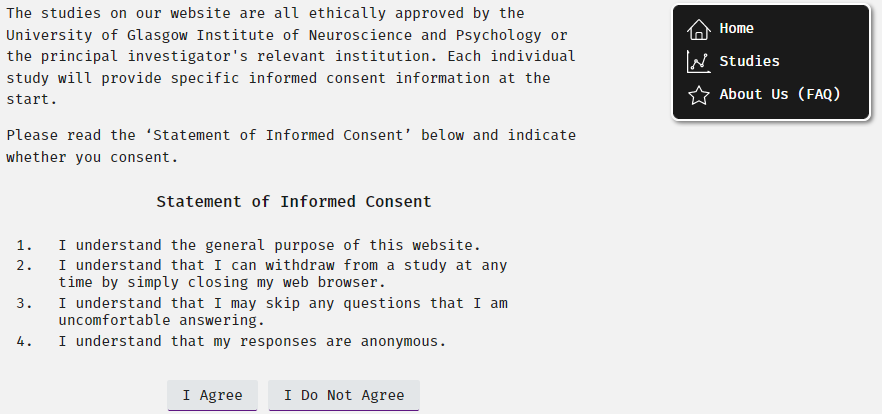
\includegraphics{images/screenshots/consent.png}

When constructing studies, you should also include your own consent
form, including all relevant information specified by your supervisor(s)
and regulatory body relevant to your work.

\section*{Codebase}\label{codebase}
\addcontentsline{toc}{section}{Codebase}

Open code for the site and installation instructions are available to
download \href{https://github.com/debruine/experimentum}{here}. This is
provided under a
\href{https://creativecommons.org/licenses/by-sa/3.0/legalcode}{CC-BY-SA
3.0} license.

The same is provided for this user guide
\href{https://github.com/RebeccaJLai/exp_manual}{here}, and under this
same
\href{https://creativecommons.org/licenses/by-sa/3.0/legalcode}{license}.
This document was authored using bookdown (Xie
\protect\hyperlink{ref-R-bookdown}{2019}). See
\href{https://bookdown.org/yihui/bookdown/}{here} for instructions on
making modifications, rendering and publishing such documents.

\section*{Acknowledgements}\label{acknowledgements}
\addcontentsline{toc}{section}{Acknowledgements}

\begin{tabular}{l|l}
\hline
Our thanks to: &  \\
\hline
Gaby Mahrholtz: & For bug hunting and fruitful discussion on workarounds and best practice.\\
\hline
Dr Niamh Stack: & For support in the development of the user guide.\\
\hline
\end{tabular}

\chapter{Quick Start Guide}\label{quick-start-guide}

\section{The Bare Essentials}\label{the-bare-essentials}

\subsection{Experiment Component
Types}\label{experiment-component-types}

\begin{tabular}{l|l|l}
\hline
Experiment Type & Response Type & DV\\
\hline
2AFC & Alternative force choice with 2 options to choose from & Binary, defaulted to 0 or 1 assigned depending on how you assign the stimuli to trials.\\
\hline
2-AFC with 8 button strength of choice & Alternative force choice between two stimuli, but with the addition of strength of preference for the choice made on an 8-point scale. & Out of 8, with 0-3 indicating strength of choice in one direction for one piece of stimuli and 4-7 indicating strength of choice in the other direction for the other piece of stimuli.\\
\hline
Labelled Buttons & Display 1, 2 or 3 stimuli items and participants respond on a scale set by the researcher. Akin to a Likert scale. & A numerical value corresponding to the values set by the researcher.\\
\hline
Slider & A sliding scale between two numerical points where the number is not displayed to participants. & Numerical, between upper and lower bounds and at increments set by the researcher.\\
\hline
X-AFC & Alternative forced choice with more than 2 options. Participants pick only one. & DV is a number which corresponds to the column the chosen stimuli item is assigned to on the stimuli assignment page, ranging from 1 to X.\\
\hline
Sorting & Participants put stimuli in order of some specified preference by dragging them into position on the screen & Number of times participants changed the order and the order the stimuli was placed in. Also provides stimuli original order of presentation.\\
\hline
Slideshow & Timed display of stimuli items where participants are only asked to watch, with no data collected or rendered. Usually used as a precursor to another component. & None.\\
\hline
\end{tabular}

\chapter{User Accounts}\label{accounts}

\section{Overview}\label{overview}

There are several account types that you can have with Experimentum,
each with its own purpose and different levels of privileges.

This chapter explains what account types exist, what they do, which type
of account you might want to have and how to change account types for
supervisors.

\hypertarget{accounttypes}{\section{Account Types}\label{accounttypes}}

\subsection{\texorpdfstring{``Guest''
Accounts}{Guest Accounts}}\label{guest-accounts}

For participants who are not required to have an account. You do not
need to be signed in but you can still take part in some experiments on
the site. When you close your browser, this account is discarded and no
longer tracked. This allows for anonymous participation in some
experiments.

\begin{warning}
If a guest participant closes their browser mid-way through a study
their progress will not be saved and the data will read as an incomplete
run.
\end{warning}

As guest users do not have a profile, we do not store their age, gender
or any other types of information about them. We suggest that you do not
place age or gender restrictions on studies where participants take part
anonymously as guests. When guests sign into a study with age or gender
restrictions, they will see a dialogue box asking them for their age and
gender.

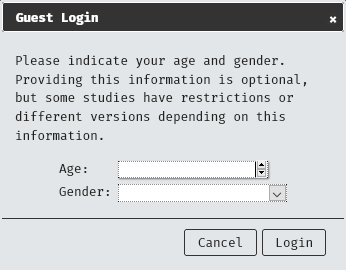
\includegraphics{images/screenshots/guest_dialogue.png}

This information is used to prevent those who should not take part from
taking part and inserted into the user information in the downloaded
data files. If you need to collect further demographic information, we
suggest constructing a demographics questionnaire component.

\begin{bug}
There is a known issue with the gathering of participant ages which has
only been observed and reported through guest type logins,
\protect\hyperlink{user_age}{see known issues for more information}.

To prevent irritrevable data loss should you experience this bug, it is
recommended that you do not rely on this method to gather ages alone.
Including a secondary age question in your demographics should give you
a backup should you need it.
\end{bug}

\subsection{\texorpdfstring{``Registered''
Accounts}{Registered Accounts}}\label{registered-accounts}

These accounts are for participants. You have created an account and
given us your date of birth and gender identification. You can
participate in studies on the site. Your participation record is
tracked, meaning that you can be linked across multiple-part studies.

Under no circumstances should you be linked across multiple studies
without your explicit permission, we will never use data to
``triangulate'' your identity. Researchers can only access your data
from their own studies, not the studies of other researchers.

\subsection{\texorpdfstring{``Student''
Accounts}{Student Accounts}}\label{student-accounts}

For students who are conducting research as part of a 3rd year
quantitative project, undergraduate dissertation, master's or doctoral
thesis. To create and run studies you must first register and then
request researcher status.

Your supervisor will be the person who changes your account status and
you can check the status of your account by looking at your account
info. When approved, students will be given ``student'' status, a
special type of research account.

You may still use this account to participate in experiments, but we
advise setting up a separate registered, non-research account for
participation to prevent serious data submissions from being removed by
other investigators.

\subsection{\texorpdfstring{``Researcher''
Accounts}{Researcher Accounts}}\label{researcher-accounts}

For staff, more senior students and anyone who may be supervising other
students using Experimentum. Follow the instructions for students as
above, but these users should set either Lisa DeBruine or Rebecca Lai as
their supervisor, who will grant them ``researcher'' status.

If you plan on supervising students using Experimentum you should set up
a researcher account to be able to oversee the construction of their
studies, share components and change studies to ``active'' before data
collection can begin.

When you have established your researcher account your name will appear
in the list of potential supervisors for students to choose from.

\begin{warning}
Supervisors should have a researcher account if they intend for their
students to use this system. If supervisors do not engage with the
system then their students will not be able to use it.

Supervision duties in this system should not be passed to another member
of staff so that you can avoid registering. Admins will not cover the
duties of the supervisor.

See the \protect\hyperlink{roles}{Supervisor Cheatsheet} for a breakdown
of the roles of the admins and the supervisors.
\end{warning}

\subsection{\texorpdfstring{``Test''
Accounts}{Test Accounts}}\label{test-accounts}

For students and staff. This account type gives you the same amount of
privileges as the registered account for participants, but any data
collected from these accounts is saved in data sets with a status of
``test''.

This allows you and other test accounts to try out your study and easily
identify and filter out which data should be excluded from the analysis.
If you wish to have a test account contact an admin to set this up.

\subsection{\texorpdfstring{``Admin''
Accounts}{Admin Accounts}}\label{admin-accounts}

For staff who assist others constructing and managing their studies
online. This is the highest level of access.

An admin account basically allows us to ``supervise'' all users,
including researcher accounts. We use this to see what is happening when
problems arise to help provide aid, not to take responsibility for
approval of status changes of students or oversee the design or
activation of studies.

\section{Registration Process}\label{registration-process}

In order to sign up to the site you will select ``Sign up'' on the top
right-hand side of the page. Once there you will be taken to a new page
as below and asked to create a username, set a password and confirm it,
provide your gender identity and birthday. Completing these steps alone
will create a ``registered'' account type.

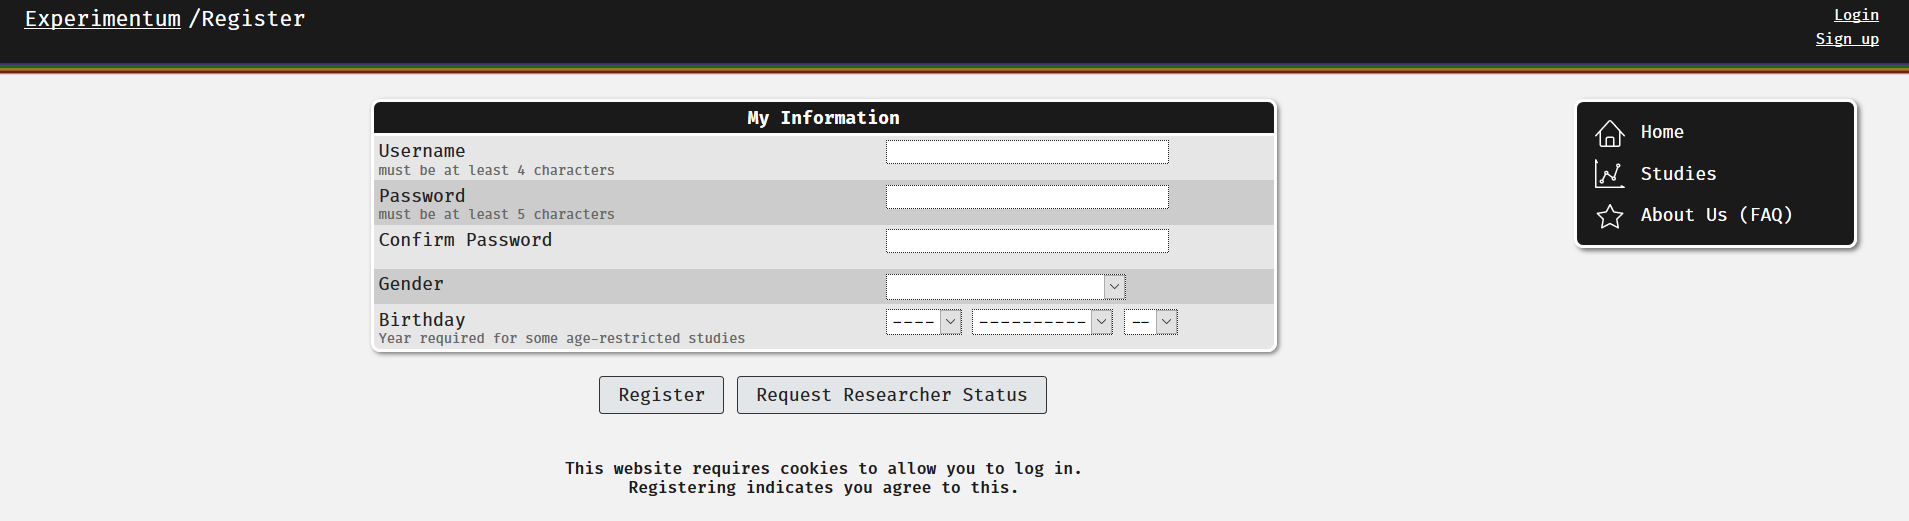
\includegraphics{images/screenshots/register.png}

With this account type you can participate in studies on the site. Your
participation record is tracked, meaning that you can be linked across
multiple-part studies. Under no circumstances will you be linked across
multiple studies without your explicit permission and we will never use
data to ``triangulate'' your identity. Researchers and students can only
access your data from their own studies, not the studies of others.

\section{Requesting Researcher
Status}\label{requesting-researcher-status}

If you are a researcher or a student who is using the site to conduct a
research project (such as a mini or maxi project, or an MSc or PhD
thesis) you will need to request permission to construct and conduct
studies. If you are a supervising member of teaching staff, you will
also need to have an account in order to supervise your students
project.

On the registration page, or the account page if you have already
registered, there is a ``Request Researcher Status'' button. When you
click on this additional fields will appear that you will need to fill
in, as below.

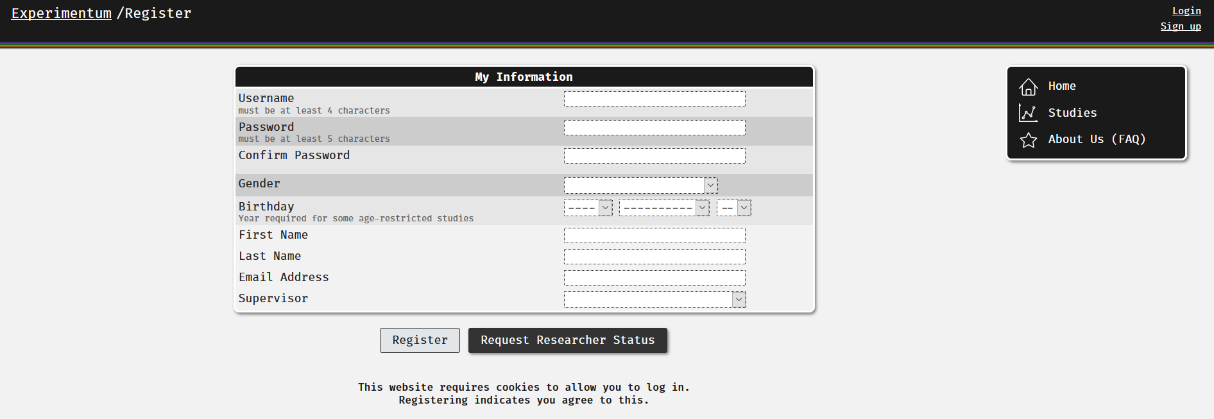
\includegraphics{images/screenshots/requesting_status.png}

You will need to provide us with your name, your email address and your
supervisor. You should use your university email address to sign up and
provide your real name so that your supervisor can more easily identify
you. If you are a student conducting a research project you should
select the member of staff supervising your project from the drop-down
menu of supervisors.

\begin{info}
If you are a supervising member of teaching or research staff, you
should request Lisa DeBruine or Rebecca Lai as your supervisor.

If you are a more senior student who is relatively self-sufficient or
you have supervising duties of your own, \emph{and your supervisor
agrees to it}, you can also request Lisa or Rebecca as your supervisor,
and we will set you as a ``researcher'' account type.

As a general rule, all students completing a research project should be
assigned ``student'' status. Some PhD students may be better off with
``researcher'' status. Such individuals should speak to their
supervisors and the admins to determine which is the best account type
for them.
\end{info}

\section{Checking your account
status}\label{checking-your-account-status}

When you first sign up your account will be the ``registered'' type and
will remain as such until your researcher status is approved. You can
check on the status of your account by selecting ``account'' from the
menu on the right-hand side of the page. Underneath the ``My
Information'' section of the page will tell you your date of
registration, number of logins and current account type.

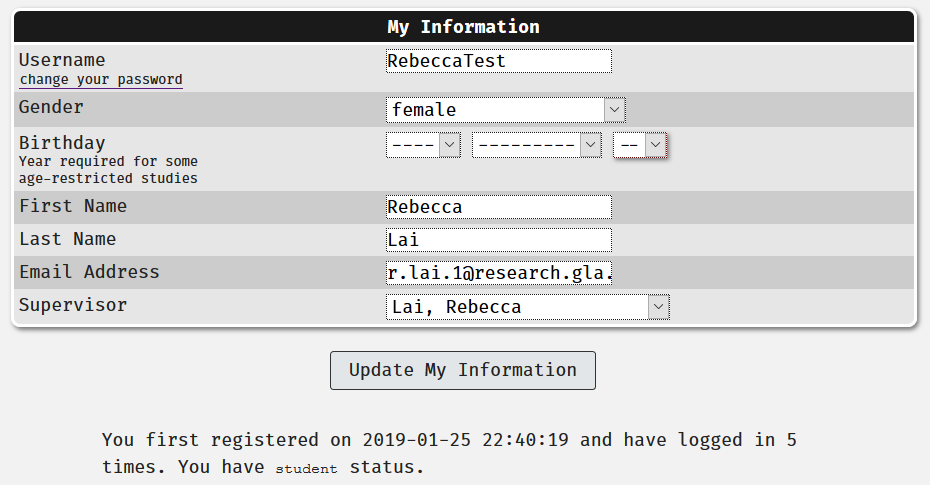
\includegraphics{images/screenshots/check_status.png}

The menu on the right also changes when you have been granted researcher
status, with a new option of ``Researchers'' available which takes you
to the study creation area of the site.

\begin{info}
If there is a delay in accepting your request you should contact your
supervisor directly and not the admin staff. It is the responsibility of
the supervisor to make changes to your access level.

If your supervisor is experiencing technical difficulties in accepting
your request, they should contact the admins directly \emph{themselves}.
Admins will not respond to a student who is requesting help on behalf of
their supervisor.
\end{info}

\section{Approving Student and Researcher Status
Requests}\label{approving-student-and-researcher-status-requests}

Supervisors have a responsibility to ensure that their students have the
status that they require to carry out their projects. This includes
assigning them sufficient permissions to construct and deploy their
studies.

If you are a supervisor and unsure as to what type of account to give a
student, refer to the \protect\hyperlink{accounttypes}{account types
section}.

Once the supervisor has ``researcher'' status they will have a new area
of the website opened to them, accessible through the researchers' link
in the menu on the right, which will contain a section called ``Admin'':

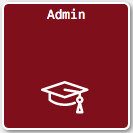
\includegraphics{images/screenshots/admin_button.png}

Clicking on this button will take them to a page with more options. To
see and make changes to the privileges of those who have requested you
as a supervisor and requested researcher status select the option
``Supervision'' from the menu.

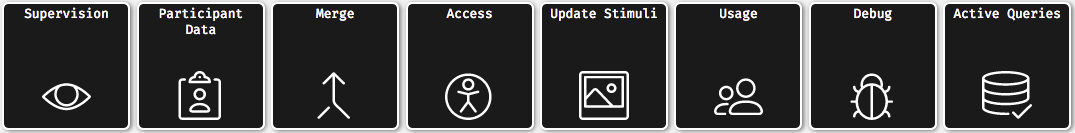
\includegraphics{images/screenshots/admin_options.png}

Here you will see a list of individuals who have requested you as a
supervisor. To change their status, select the appropriate account type
from the right-most drop-down menu under the column ``Status''.


\includegraphics{images/screenshots/status_bar.png}

The account you are making changes to will have to log out and back in
again to be updated with their new permissions. When you press ``Send''
an email will be sent to the student to inform them of the status
change.

\begin{bug}
There is a known issue with changing the statuses of research accounts
regarding accounts not being found by the system,
\protect\hyperlink{notfound}{see here}
\end{bug}

\hypertarget{stimuli}{\chapter{Stimuli}\label{stimuli}}

\begin{warning}
Things to add:

\begin{itemize}
\tightlist
\item
  Creating image stimuli will need to have it's own section, this can
  incorporate individual image conversion and resizing via GIMP
\end{itemize}
\end{warning}

\section{Overview}\label{overview-1}

This chapter will cover how to upload your own stimuli, tips on naming
conventions for the easiest possible way to assign stimuli to trials,
accepted file formats and a rough guide to how to convert to the
required formats.

\begin{warning}
Remember that not all image, video and audio files are free for use.
Check the license and terms of use of the images before you save, edit
or copy and paste them.
\end{warning}

\section{Accepted File Formats}\label{accepted-file-formats}

Experimentum uses what we hope to be the most universally applicable
file formats to deliver your study.

These are the file formats that can be successfully displayed through
the site. Please ensure that you conform to these types as others may
not be tolerated by the system.

\begin{tabular}{l|l}
\hline
Stimuli Type & Accepted Formats\\
\hline
Images & JPEG, GIF and PNG\\
\hline
Audio & MP3\\
\hline
Video & M4V\\
\hline
\end{tabular}

\section{Naming Conventions}\label{naming-conventions}

In order to make the process of assigning stimuli to trials as easy as
possible it is recommended that you establish a systematic way of
assigning names to files.

The stage of assigning stimuli to trials goes much faster and smoother
if you can search for the stimuli files names using some sort of common
text string in the names of the files.

For example, here I have 24 stimuli items. These are stylized face
images of both mal and female gender (Mooney
\protect\hyperlink{ref-mooneys}{1957}). I have named them using the
convention ``mooneyxn.jpg'', where x is either m or f (for male and
female) and n for the number of the pair that I will present them in:

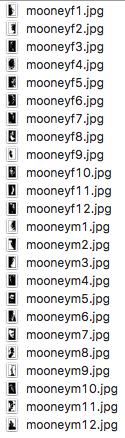
\includegraphics{images/screenshots/stim_1.png}

This systematic naming helps in searching for your stimuli later when
you come to assign them to trials. Here I can use the search box to find
all stimuli containing the string ``mooneyf''. I can then assign them to
one of two images displayed in each trial of this two alternative forced
choice (2AFC) experiment below:

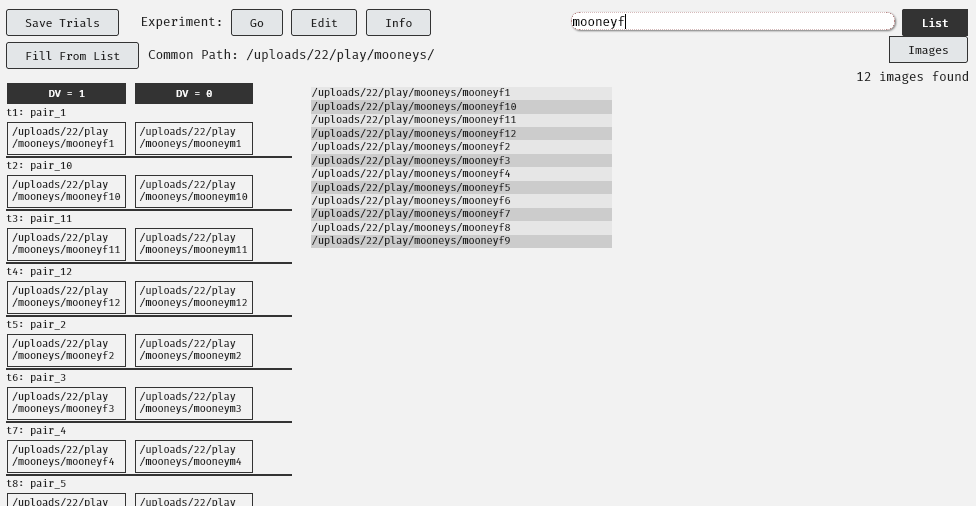
\includegraphics{images/screenshots/stim_3.png}

I can also search for ``mooneym'' and repeat the process for the other
image for the male faces.

It is also beneficial to store their names in an Excel spreadsheet. Here
I have stored them in pairs under column headers. I can use this later
when assigning them to trials. I have also assigned trial names; this
will come in handy should I need to know which trial each data point
refers to in my analysis.

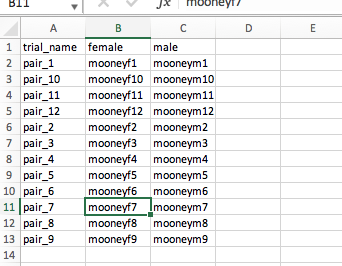
\includegraphics{images/screenshots/stim_2.png}

This example above is where each male face will be compared to a
corresponding female face in a trial with two images. You may have more
or less than two stimuli items per trial and your spreadsheet should
vary accordingly.

\section{Pre-Processing}\label{pre-processing}

In order to get your stimuli up with the minimal amount of fuss, please
ensure that you do any required pre-processing.

\subsection{Images}\label{images}

Images should be of uniform size and of the correct file formats before
uploading. The following information is but one way that you can amend
your files to the correct format and resolution for the site. There may
be other ways to acheive the same goal.

If you do not resize your stimuli to the appropriate size you might find
inconsistencies in the presentation of your stimuli that could act as a
confounding factor in your experiments:

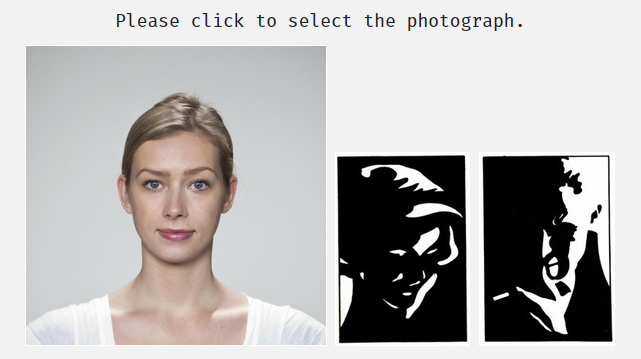
\includegraphics{images/screenshots/not_pre_processed.png}

\subsubsection{Individual Images}\label{individual-images}

If you need to work on a single image, such as resizing, or need to
create your own images, then GNU Image Manipulation Program (``GIMP'',
The GIMP Development Team \protect\hyperlink{ref-gimp}{2019}) may be a
good choice of software for you.

\paragraph{Converting Images}\label{converting-images}
\addcontentsline{toc}{paragraph}{Converting Images}

GIMP is a free software that allows you to modify and export image files
to a variety of file formats.


\includegraphics{images/screenshots/gimp.png}

This software was developed as a free and open source equivalent to
photo-editing software such as Adobe Photoshop and can achieve very
complex tasks. However, there are only 3 basic operations that you
should be able to perform in GIMP order to convert your images to the
correct formats. More complex operations are beyond the scope of this
tutorial, but there are plenty of resources online should you choose to
want to look them up.

If there are any further instructions that would prove helpful please
file an issue
\href{https://github.com/RebeccaJLai/exp_manual/issues}{here} describing
what you want me to include in future versions of the manual.

\paragraph{Importing Images}\label{importing-images}
\addcontentsline{toc}{paragraph}{Importing Images}

There are a number of ways that you can import images into GIMP.

\subparagraph{File \textgreater{} Open}\label{file-open}
\addcontentsline{toc}{subparagraph}{File \textgreater{} Open}

This is the simplest way to open an image file in GIMP.

Open the software first from your Start Menu or Launchpad. Then click on
File \textgreater{} Open\ldots{}

***** image in here

A dialogue box will appear from which you can navigate to the location
of the file you are attempting to open and select it. Click Open and the
file will appear in a new tab.

***** image in here

\subparagraph{\texorpdfstring{``Open
With''}{Open With}}\label{open-with}
\addcontentsline{toc}{subparagraph}{``Open With''}

If you already have the image file saved on your PC, you can navigate to
the file's location through your file explorer or finder and right click
on it. Select ``Open With'' in the menu that pops up. This will open the
GIMP GUI and should open a new tab with that image inside it.

On some machines GIMP will not be automatically recognised as a type of
software associated with image files. In this case you will need to
select ``Choose another app'' and navigate to the executable file for
GIMP (location may vary depending on machine and operating system type).

It is not advisable to permanently change all image files to be
associated with GIMP, as the software can run slowly and sometimes you
only want to view an image in a photo browser, not edit it.

\subparagraph{Edit \textgreater{} Paste as\ldots{} \textgreater{} New
Image}\label{edit-paste-as-new-image}
\addcontentsline{toc}{subparagraph}{Edit \textgreater{} Paste as\ldots{}
\textgreater{} New Image}

Finally, if the image file is not saved on your computer you can copy it
to the clipboard and paste it directly into GIMP. Do this by going to
Edit \textgreater{} Paste as\ldots{} \textgreater{} New Image.

This will create a new image in GIMP that is not yet saved. I recommend
saving immediately in the first instance and periodically thereafter.

\paragraph{GIMP File Format}\label{gimp-file-format}
\addcontentsline{toc}{paragraph}{GIMP File Format}

The file extension of files created in GIMP will be \texttt{.xcf}. These
types of files allow for saving of \texttt{image\ layers} and
\texttt{text\ path\ information}, allowing you to have an image made of
multiple layers and with text that can be edited at a later point.

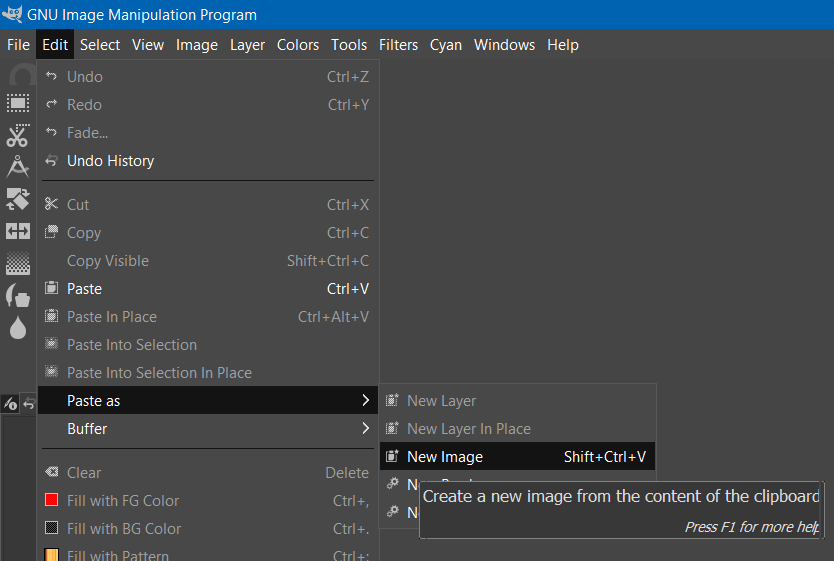
\includegraphics{images/screenshots/paste_as_new_gimp.png}

\begin{info}
Saving images with layers and text path information could come in handy
if you are generating your own image stimuli which features small
changes (such as different words), but remains mostly the same (same
background colour, size, fonts, etc).

In this case you could save a layer or export a different .GIF, .JPG or
.PNG from the same .XCF file for each change that you need to make.
\end{info}

\paragraph{Changing Image Size}\label{changing-image-size}
\addcontentsline{toc}{paragraph}{Changing Image Size}

Images that are too large can be resized in the
\texttt{\textless{}img\textgreater{}} html tag to fit into a smaller
space but if your image is too large you could be using more memory than
would be required to store your images on the server.

This may have a knock on effect in the stimuli loading times.

Rather than consume excess bandwidth it is adviable to size the images
down prior to uploading them on to the server.

To resize the image (and all layers and items contained within) click on
the menu Image and press ``Scale Image\ldots{}''. This dialoue box will
come up:

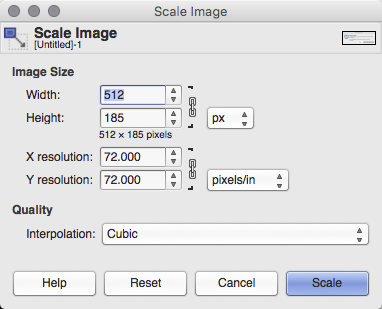
\includegraphics{images/screenshots/scale_image.png}

The image size defaults to \texttt{px}, or pixels. The height and the
weight are by default linked together (as demonstrated by the chain
symbol to the right of the two boxes). When linked changing either the
height or the width will keep the image to the same aspect ratio (the
proportions of the sizes). You may unlink the aspect ratio by clicking
on the chain. When unlinked the chain will appear as broken.

Linking these helps you avoid distortion that might happen if you resize
one dimension only, which might elongate/shorten the other dimension and
make it look funny. It also allows you to make images to fit in a
specific space in your study. For example, this word completion task
where images are used instead of text:

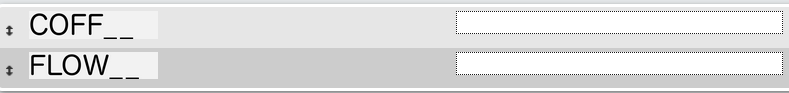
\includegraphics{images/screenshots/image_size_example.png}

I have used images in the question field of a mixed questionnaire, as
the blank spaces are more apparent to the participants. I have also
limited their size to 25px to ensure that they do not seem too oversized
in comparison to the text entry fields next to them.

\paragraph{Exporting Images}\label{exporting-images}
\addcontentsline{toc}{paragraph}{Exporting Images}

GIMP is capable of exporting GIF, JPEG and PNG file formats.

To export your image go to File \textgreater{} Export As. You will then
be asked to enter a file name in the text box at the top of the dialogue
box that opens up.

You can specify the type of file by typing the file extension at the end
of the file name, ``.gif'', ``.jpg'' or ``.png'' for each of the
aforementioned file types respectively.

Once you have done this, press the ``export'' button at the bottom of
the dialogue box.

You may be asked to specify compression options after pressing the
button. This is just to ask how much (if any) quality you are willing to
sacrifice to save on the size of the file.

This is an example from a PNG file. This image was compressed with the
default options. As you can tell the quality is good, but the image is
not very rich. A richer image with higher levels of variation in the
pixels may do worse that this one with the same level of compression.

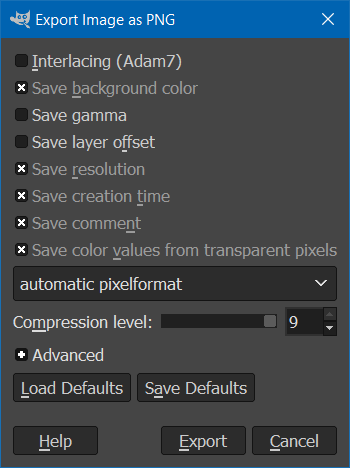
\includegraphics{images/screenshots/export_1.png}

When exporting JPEG files you will be asked to select the quality as a
percentage, not compression level. The higher the percentage the higher
the quality and the less compression being done.

Experiment with the levels of comrpression in the image and examine the
outputs carefully for any artifacts in the images resulting from the
compression process. If you find the quality lacking, lower the amount
of compression allowed and try again until you find the level
appropriate for your images.

These images are saved as JPEG, and are at 100\%, 50\% and 0\% quality.
This gives file sizes of 76KB, 9KB and 2KB respectively:

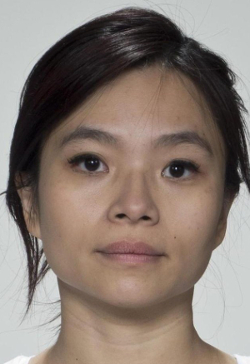
\includegraphics{images/screenshots/087_03_min.jpg}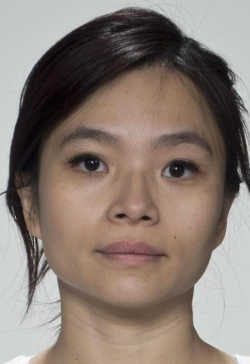
\includegraphics{images/screenshots/087_03_mid.jpg}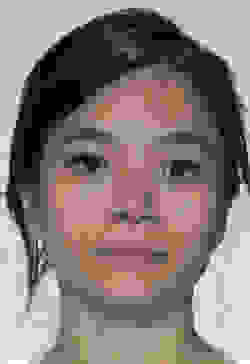
\includegraphics{images/screenshots/087_03_max.jpg}

The first is 100\% quality, no compression. The second has minimal
pixelation artifacts around the periphery of the face, neck, hair and
some issues with the skin texture in places. It also seems (to my office
mates and I at least) that the skin tone is a little yellower in image
2. Number 3 is unusable for the vast majorit of purposes.

The level of compression that you choose will be a compromise between
what the system can successfully deliver and what the level of
compression does to the images that you are using.

\subsubsection{Batch Images}\label{batch-images}

If you have pre-existing stimuli that need to be resized or converted to
another format you may want to use IrfanView (Irfan Skiljan
(\protect\hyperlink{ref-irfanview}{2019})).


\includegraphics{images/screenshots/irfanview_1.png}

IrfanView is a fast, compact image viewer and editor for Windows XP,
Vista, 7, 8 and 10 available in 32 and 64 bit versions.

\paragraph{Batch Conversion}\label{batch-conversion}
\addcontentsline{toc}{paragraph}{Batch Conversion}

\begin{info}
You can resize and convert images at the same time by setting the
appropriate options in one process.
\end{info}

If you need to convert images to JPG, GIF or PNG in bulk, you can do
this easily.

First, ensure that all of your files are in the same folder. Open
IrfanView and go to ``File'' \textgreater{} ``Batch Conversion/Rename'':

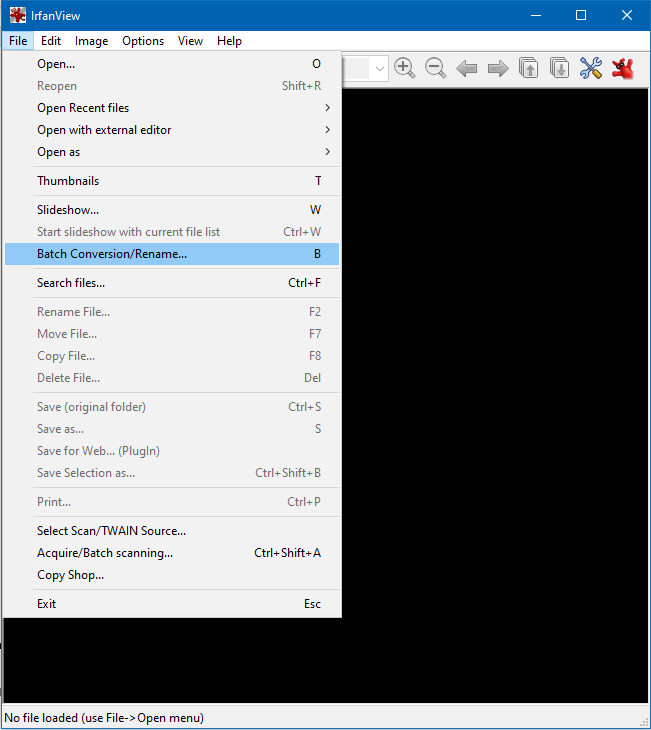
\includegraphics{images/screenshots/irfanview_2.png}

This will open the Batch conversion dialogue:

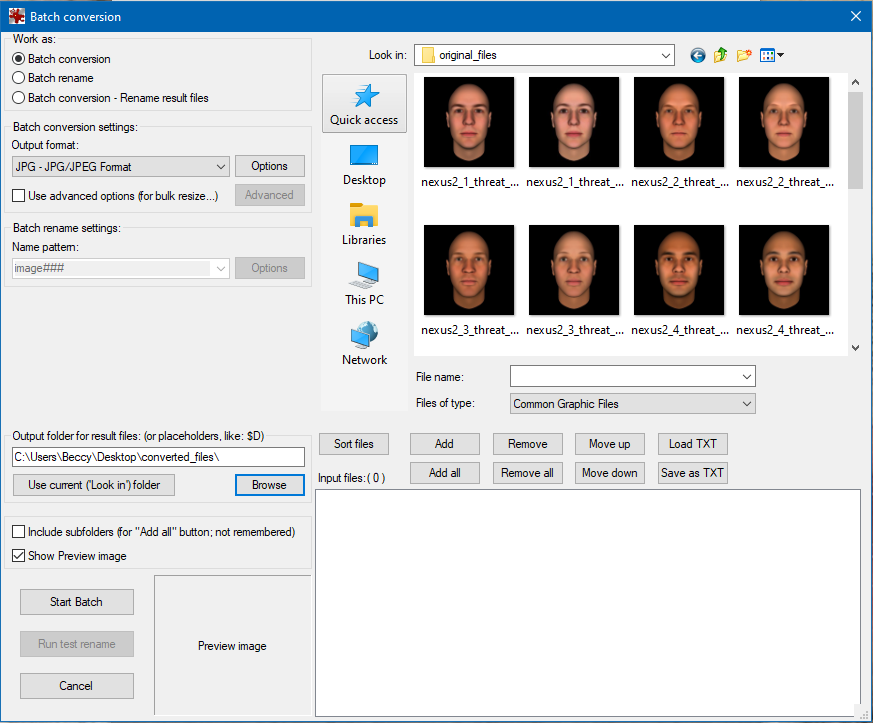
\includegraphics{images/screenshots/irfanview_3.png}

In the top left, ensure that batch conversion and the intended output
format are selected:

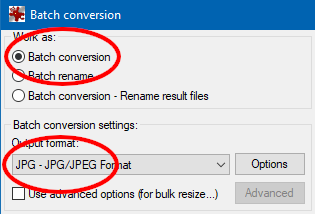
\includegraphics{images/screenshots/irfanview_4.png}

In the top centre, use the ``Look in:'' part of the window to naviagte
to the folder in which the images to be converted are stored. Highlight
the images to be converted and press ``Add'', or if you are converting
all the files in the folder, press ``Add all'':

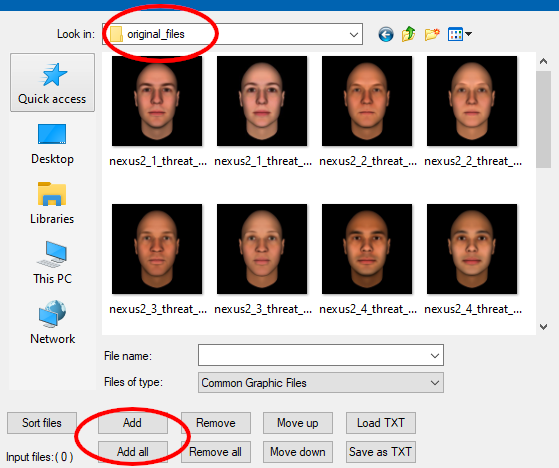
\includegraphics{images/screenshots/irfanview_5.png}

The bottom box showing ``Input files'' should now be populated with your
files. Check that the count (shown in brackets) corresponds to the
number of items that you expect:

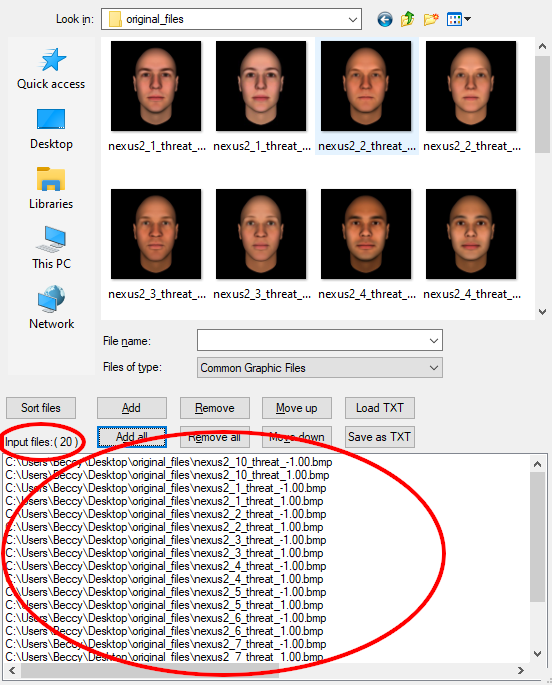
\includegraphics{images/screenshots/irfanview_5a.png}

To the left of this select the output folder. This is where the
converted image files will be placed. It is best to create a new folder
to keep the types of image separate:

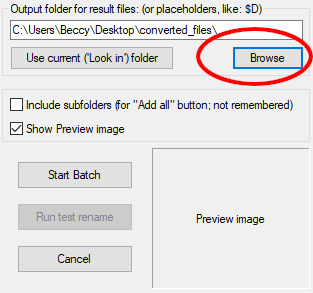
\includegraphics{images/screenshots/irfanview_6.png}

This is the file browser dialogue that you will see. Find the folder you
want to store the converted files in and press ``OK'':

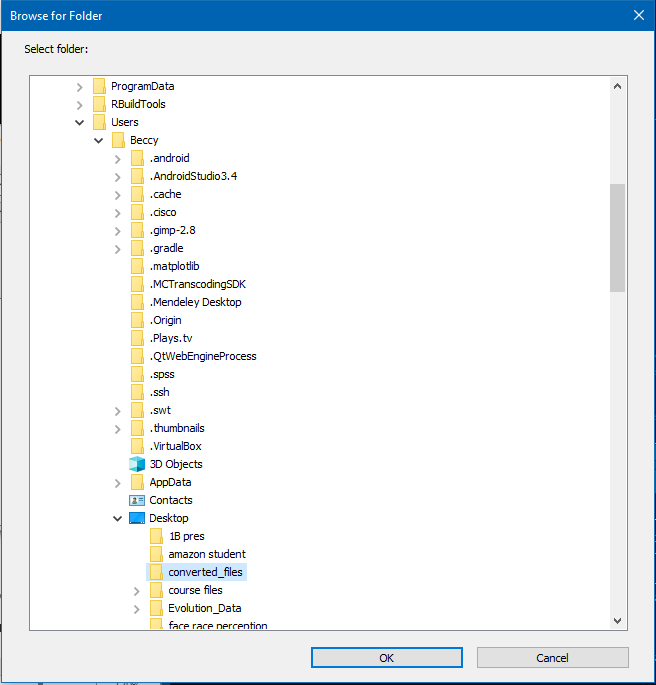
\includegraphics{images/screenshots/irfanview_6a.png}

Click ``Start Batch'' to begin the conversion process:

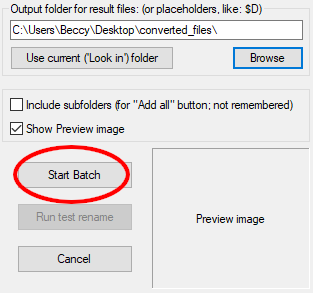
\includegraphics{images/screenshots/irfanview_7.png}

You will be shown a dialogue box showing the processing. Once conversion
is complete you will be shown a one line summary. you can now press
``Exit batch'' if you are finished:

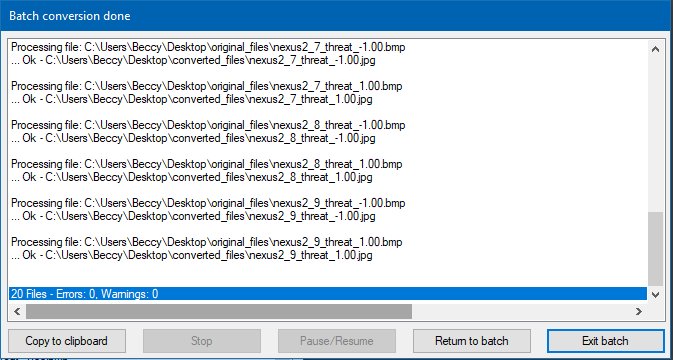
\includegraphics{images/screenshots/irfanview_7a.png}

Double check that your output files are correct after you have run the
batch processing by navigating to them using your file system browser.

\paragraph{Batch Resize}\label{batch-resize}
\addcontentsline{toc}{paragraph}{Batch Resize}

\begin{info}
You can resize and convert images at the same time by setting the
appropriate options in one process.
\end{info}

If your images are the wrong size you can also resize the images in bulk
too.

Select the input files and output folder as explained above in the
previous section .Access the ``Bulk Conversion/Rename'' dialogue again
from the file menu:

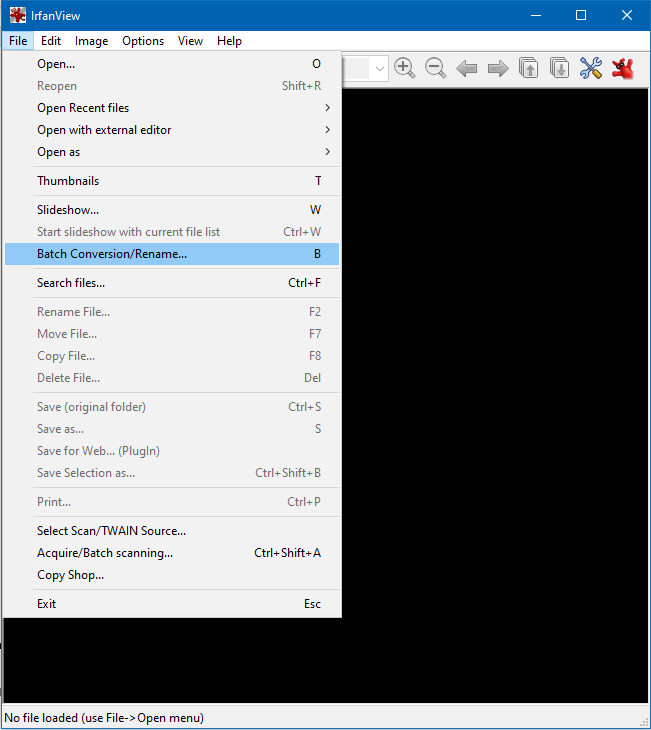
\includegraphics{images/screenshots/irfanview_2.png}

In the dialogue, select ``Use advanced options (for bulk resize)'' and
then press the ``Advanced'' button:

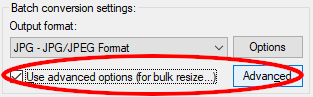
\includegraphics{images/screenshots/irfanview_8.png}

Use the ``Resize'' section to set a new size:

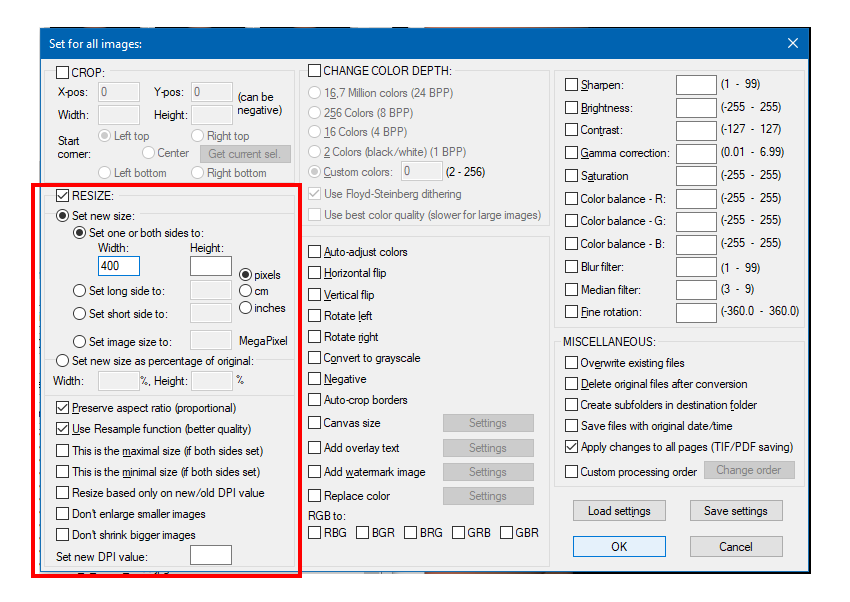
\includegraphics{images/screenshots/irfanview_9.png}

Here I have reduced my images from 1024*1024 pixels to 400*400 pixels
(as the dimensions match on each side).

Press OK to return to the previous dialogue where, if you have set the
other options as indicated above, you can press the ``Start Batch''
button:

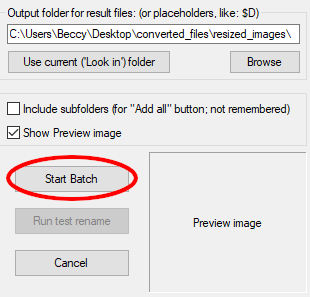
\includegraphics{images/screenshots/irfanview_10.png}

You will get the processing dialogue showing the processing and the
completion message should it all go well:

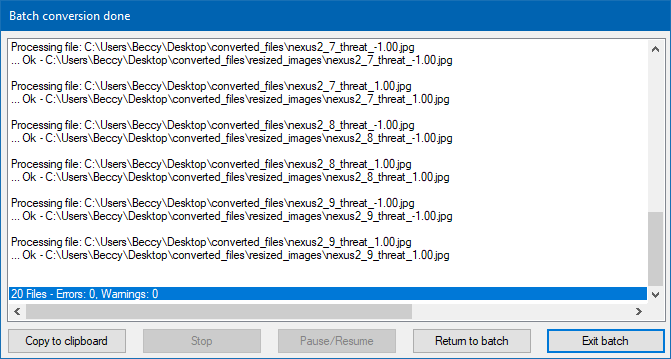
\includegraphics{images/screenshots/irfanview_10a.png}

You can use the other options to achieve other goals, but this is the
simplest way to resize images.

\subsection{Audio}\label{audio}

Since Experimentum requires auditory stimuli to be uploaded as .mp3
files, here is an easy way to convert audio files (like .wav) to mp3s
using Audacity's batch-processing feature.


\includegraphics{images/screenshots/audacity_logo.png}

Audacity is free and open source cross-platform software which can be
used to record (with suitable microphone), import, edit and export audio
files in many different formats. This is also software that both the
Voice Perception Lab and Face Research Lab use in their research.

Here you will find the minimal instructions that will allow you to
convert your audio files to \texttt{.mp3} format in Audacity. For the
full user guide see
\href{https://manual.audacityteam.org/index.html}{here}.

\subsubsection{Audacity 2.1.2}\label{audacity-2.1.2}

If you are still on an older version of audacity, go to File
\textgreater{} Edit Chains

There is already a chain set up for mp3 conversion, which contains 3
steps: Normalising, exporting as mp3, and an END process.

Normalisation is a process by which you standardise the aplitude of the
audio signal. If you have recorded your own stimuli you will need to
normalise it first to ensure that no audio clips are excessively loud or
quiet in comparison to the others.

If you are using stimuli sourced from elsewhere it may already be
normalised. In this case, highlight the first step of the chain and
press delete.

All you should have in the chain ``MP3 Conversion'' is 1. ExportMP3, and
2. -END-. Click ``OK'' to save the chain.

Now, go to File \textgreater{} Apply Chain\ldots{}

\ldots{} select MP3 Conversion, and confirm with ``Apply to
Files\ldots{}''

Locate the files you want to convert into mp3s from the folder on your
computer, select all, and confirm with ``Open''.

The selected files will then be converted into mp3s. You will find an
additional folder called ``cleaned'' within the folder your original
files are located in.

Content of the folder ``cleaned'':

\subsubsection{Audacity 2.3.0}\label{audacity-2.3.0}

Audacity version 2.3.0 changed the batch-processing process, relabelling
chains as ``Macros''. The menu for accessing the Macros got relocated to
Tools \textgreater{} Macros\ldots{}

The following steps are fairly similar to older versions of audacity.

Within the macros you will find one already labelled ``MP3 Conversion''.
In the window ``Edit Steps'', select the normalise step (Num 01) and
delete it if you have already normalised the amplitude of the stimuli
you are using.

Make sure you have only the steps ``ExportMP3'' and ``-END-'' left in
your macro; then click on ``Files\ldots{}''

Locate the files you want to convert to mp3s on your computer, select/
highlight all of them, and confirm with ``Open''.

There might be a warning message popping up asking you for an input
method. Select the safer or faster option according to your personality,
and confirm with ``OK''.

Once the process is done, you can find the converted mp3s in a separate
folder called ``cleaned'' that is located within the folder of your
original files.

Content of the folder ``cleaned'':

\subsection{Video}\label{video}

Experimentum required video stimuli to be uploaded in \texttt{.m4v}
format. Here is a short tutorial based upon Reed
(\protect\hyperlink{ref-m4vconv}{2016})

These are similar to the files with \texttt{.mp4} extensions -- the main
difference is that \texttt{.m4v} files are Digital Rights Management
(DRM) copyright protected and are mostly used by Apple.

If you have a Windows laptop, you can manually change \texttt{.mp4}
video files to \texttt{.m4v} ones without downloading additional
software sometimes.

\begin{warning}
This process will only work when the videos are not already copyrighted.
Remember that not all files are free to use!

This could mean that any file you attempt to convert that has copyright
protection will not run again on your computer's standard video viewer
so be sure to make copies \textbf{if you have permission to use it} in
case the conversion fails.
\end{warning}

First go to the file where you have placed your videos. If not already
showing, make sure you change the settings so that you can see the file
extension.

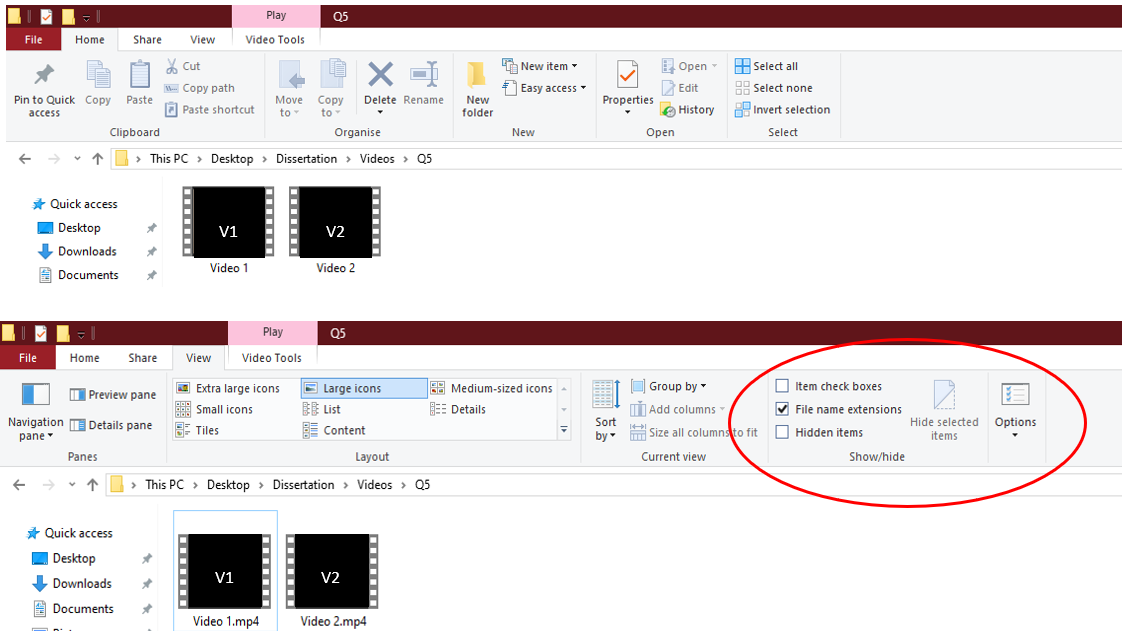
\includegraphics{images/screenshots/video_conv_1.png}

To include the file extension in the name, click on View \textgreater{}
File name extensions and check the box or Options \textgreater{} Change
folder and search options \textgreater{} View \textgreater{} Advanced
settings and uncheck Hide extensions for known file types. You will see
that it now says ``videoname''.mp4

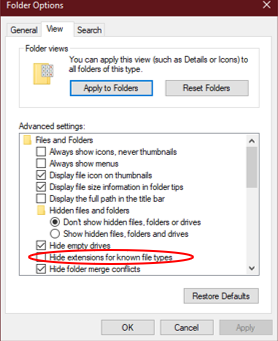
\includegraphics{images/screenshots/video_conv_2.png}

You can change this by simply renaming the file to ``videoname''.m4v and
clicking ``Yes'', This should make it compatible with the Experimentum
website however it may not work if the file is copyright protected. This
should not be an issue if you are creating your own custom video
stimuli.

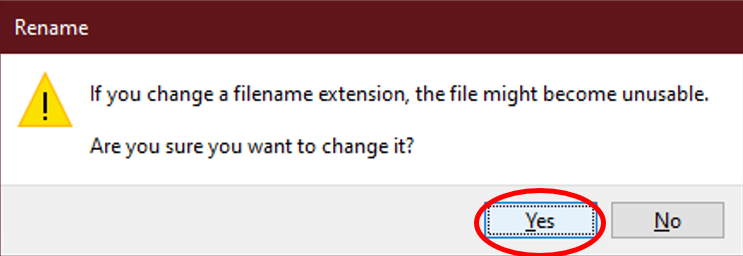
\includegraphics{images/screenshots/video_conv_3.png}

\begin{warning}
The presentation of video stimuli is designed for short snippets, rather
than longer clips.

For optimal performance keep your file sizes in the 2-3Mb range.

If you require longer videos you may need to host the content externally
(such as on YouTube) and use HTML to embed it into a questionnaire
component.
\end{warning}

\hypertarget{stimupload}{\section{Uploading Stimuli}\label{stimupload}}

For the purposes of demonstration of uploading stimuli I will be using
The MR2 face stimuli set (Strohminger et al.
\protect\hyperlink{ref-mr2}{2016}), which is available to download and
use under a Creative Commons License.

\section{Using Stimuli}\label{using-stimuli}

\hypertarget{htmlstim}{\subsection{Using Stimuli Items In
Questionnaires, Set and Component Introductions}\label{htmlstim}}

You may use stimuli items uploaded to the server in questionnaire
introduction sections and individual question fields by using either
Markdown or HTML syntax.

\begin{Shaded}
\begin{Highlighting}[]
\CommentTok{# The HTML code}
\OperatorTok{<}\NormalTok{img src=}\StringTok{"image file path goes here with extension"}\OperatorTok{>}
\StringTok{  }
\CommentTok{# The Markdown code}
\OperatorTok{!}\NormalTok{[](image file path goes here with file extension)}
\end{Highlighting}
\end{Shaded}

The image file path can be found by navigating to Researchers
\textgreater{} Stimuli \textgreater{} Uploads, selecting the folder name
you gave it when you uploaded it and then the image:

\begin{figure}
\centering
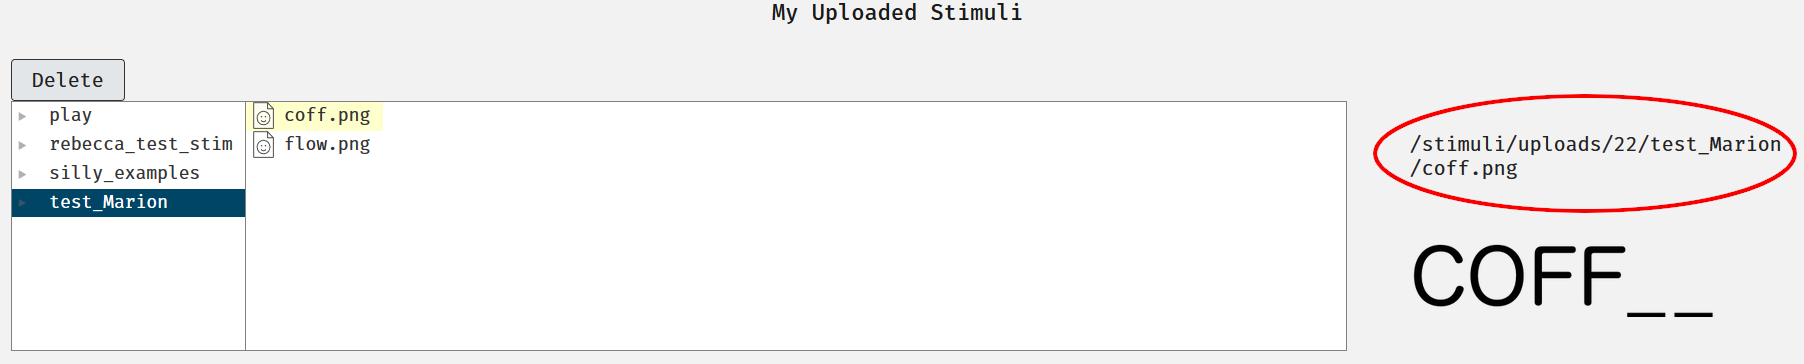
\includegraphics{images/screenshots/img_file_path.png}
\caption{}
\end{figure}

The image file path is on the right hand side of the page above where
the image is displayed.

For additional information on using HTML code please see this tutorial
on \href{https://www.w3schools.com/html/}{W3Schools}.

\subsection{Assigning Stimuli to Experimental
Trials}\label{assigning-stimuli-to-experimental-trials}

Assigning stimuli to trials is a fundamental part of the process of
constructing experimental components so this is covered in the section
regarding experimental components
\protect\hyperlink{assignstimexp}{here}.

\subsection{Using Stimuli in
Questionnaires}\label{using-stimuli-in-questionnaires}

You can link to stimuli in your questionnaires too. Please read the
section in the \protect\hyperlink{assignstimquest}{questionnaires} about
using stimuli in conjuction with your questionnaires.

\chapter{Planning Your Project}\label{planning-your-project}

\section{Overview}\label{overview-2}

\section{Planning Your Project}\label{planning-your-project-1}

\section{Implementing Your Plan}\label{implementing-your-plan}

\subsection{Individual Components}\label{individual-components}

\subsection{Sets and Supersets}\label{sets-and-supersets}

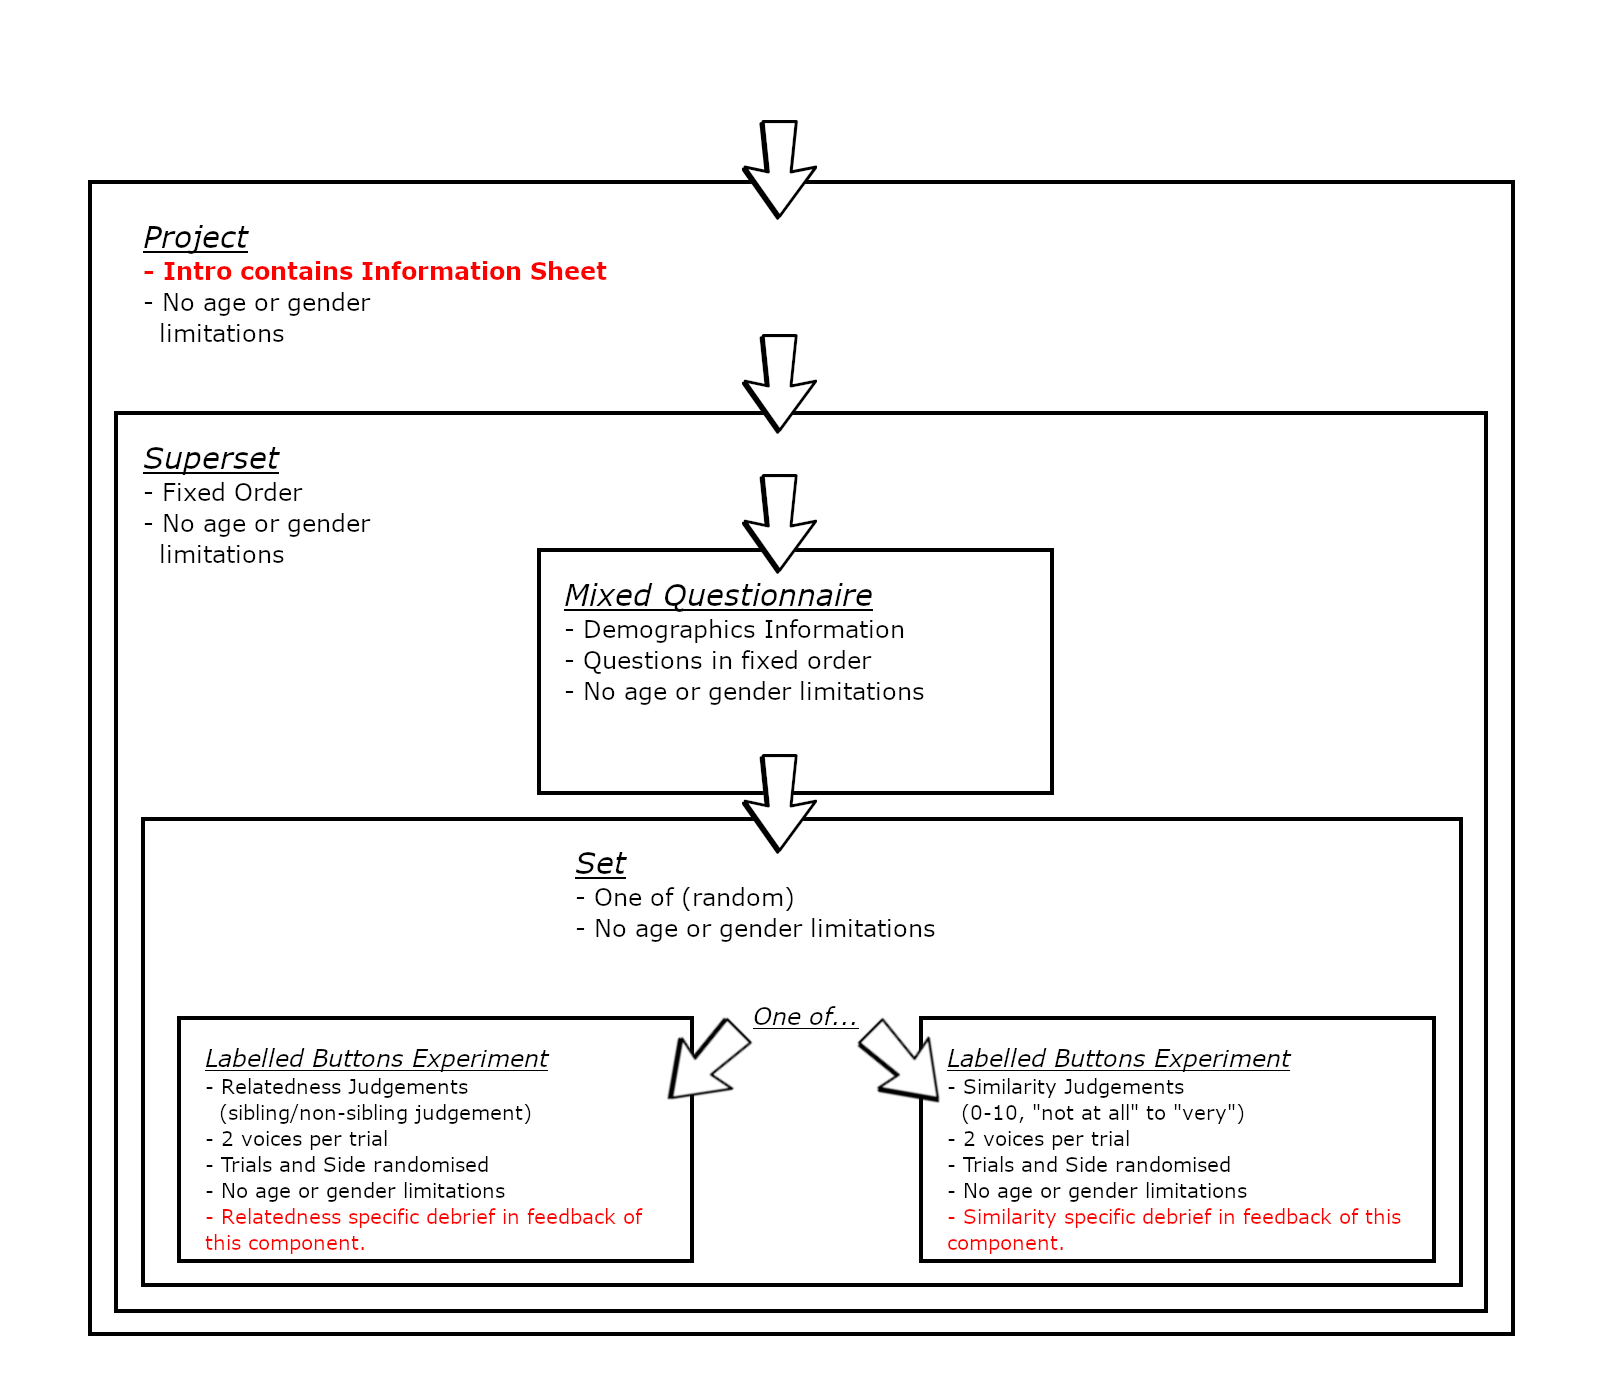
\includegraphics{images/screenshots/structure.png}

\subsection{Information Sheet}\label{info_sheet}

The information sheet should normally be placed in the introduction
section on the project information page (the box labelled ``Intro''), as
below:

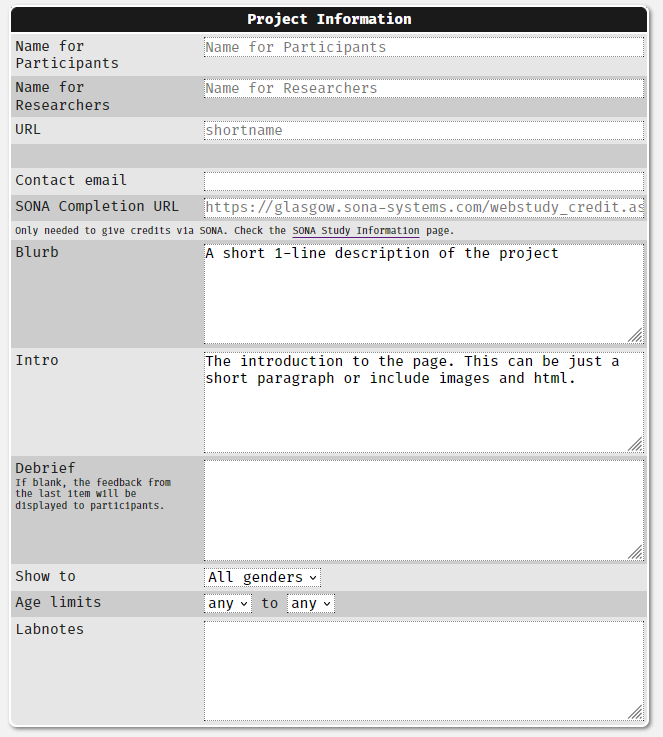
\includegraphics{images/screenshots/proj_3.png}

It can be formatted with Markdown or HTML tags. If you use HTML tags,
ensure that your opening and closing tags are matched to prevent data
recording errors. Here is the flowchart view of where the information
sheet should be placed, highlighted in red:

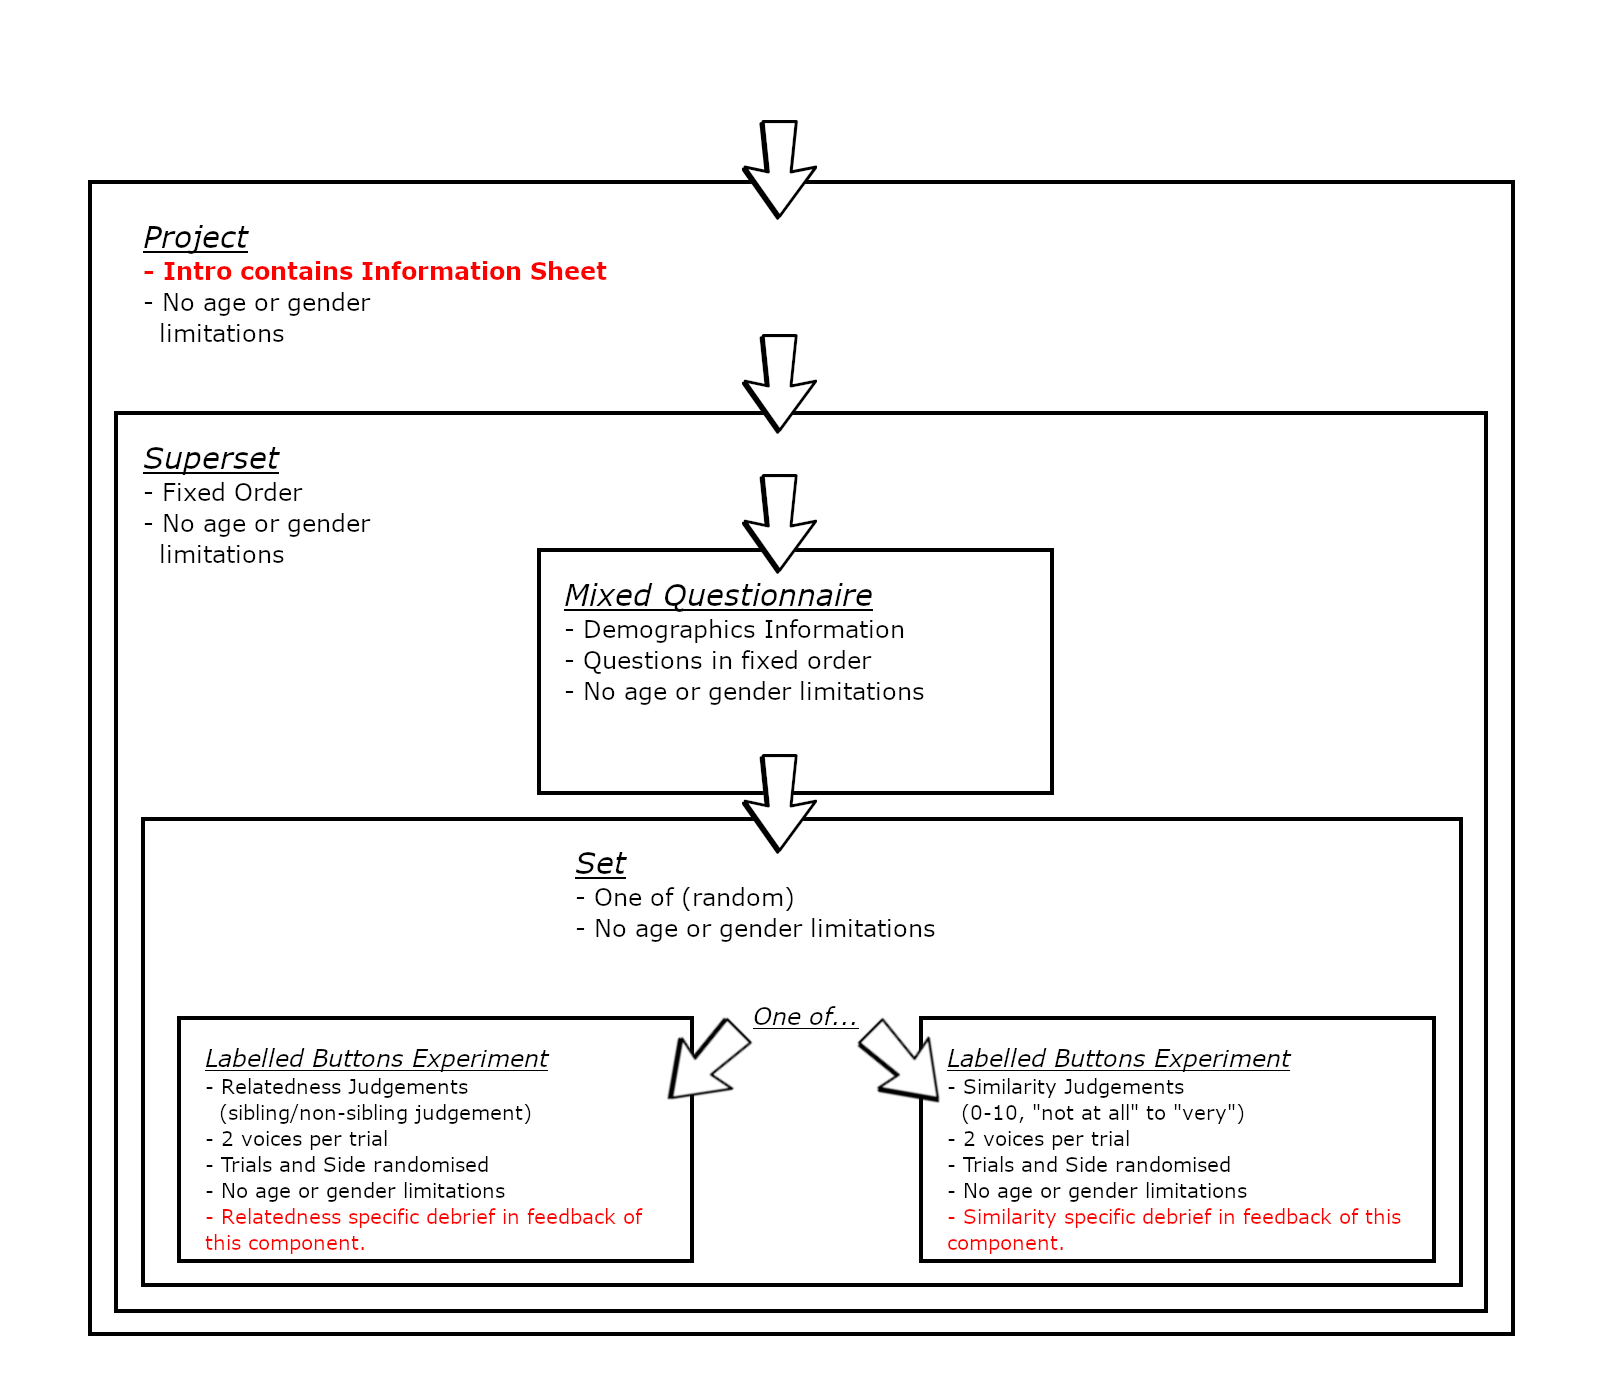
\includegraphics{images/screenshots/structure.png}

\hypertarget{debrief}{\subsection{Debriefing}\label{debrief}}

Your debriefing information should be placed in the highest possible
level component possible. In most cases this will be the top-most
superset within the project

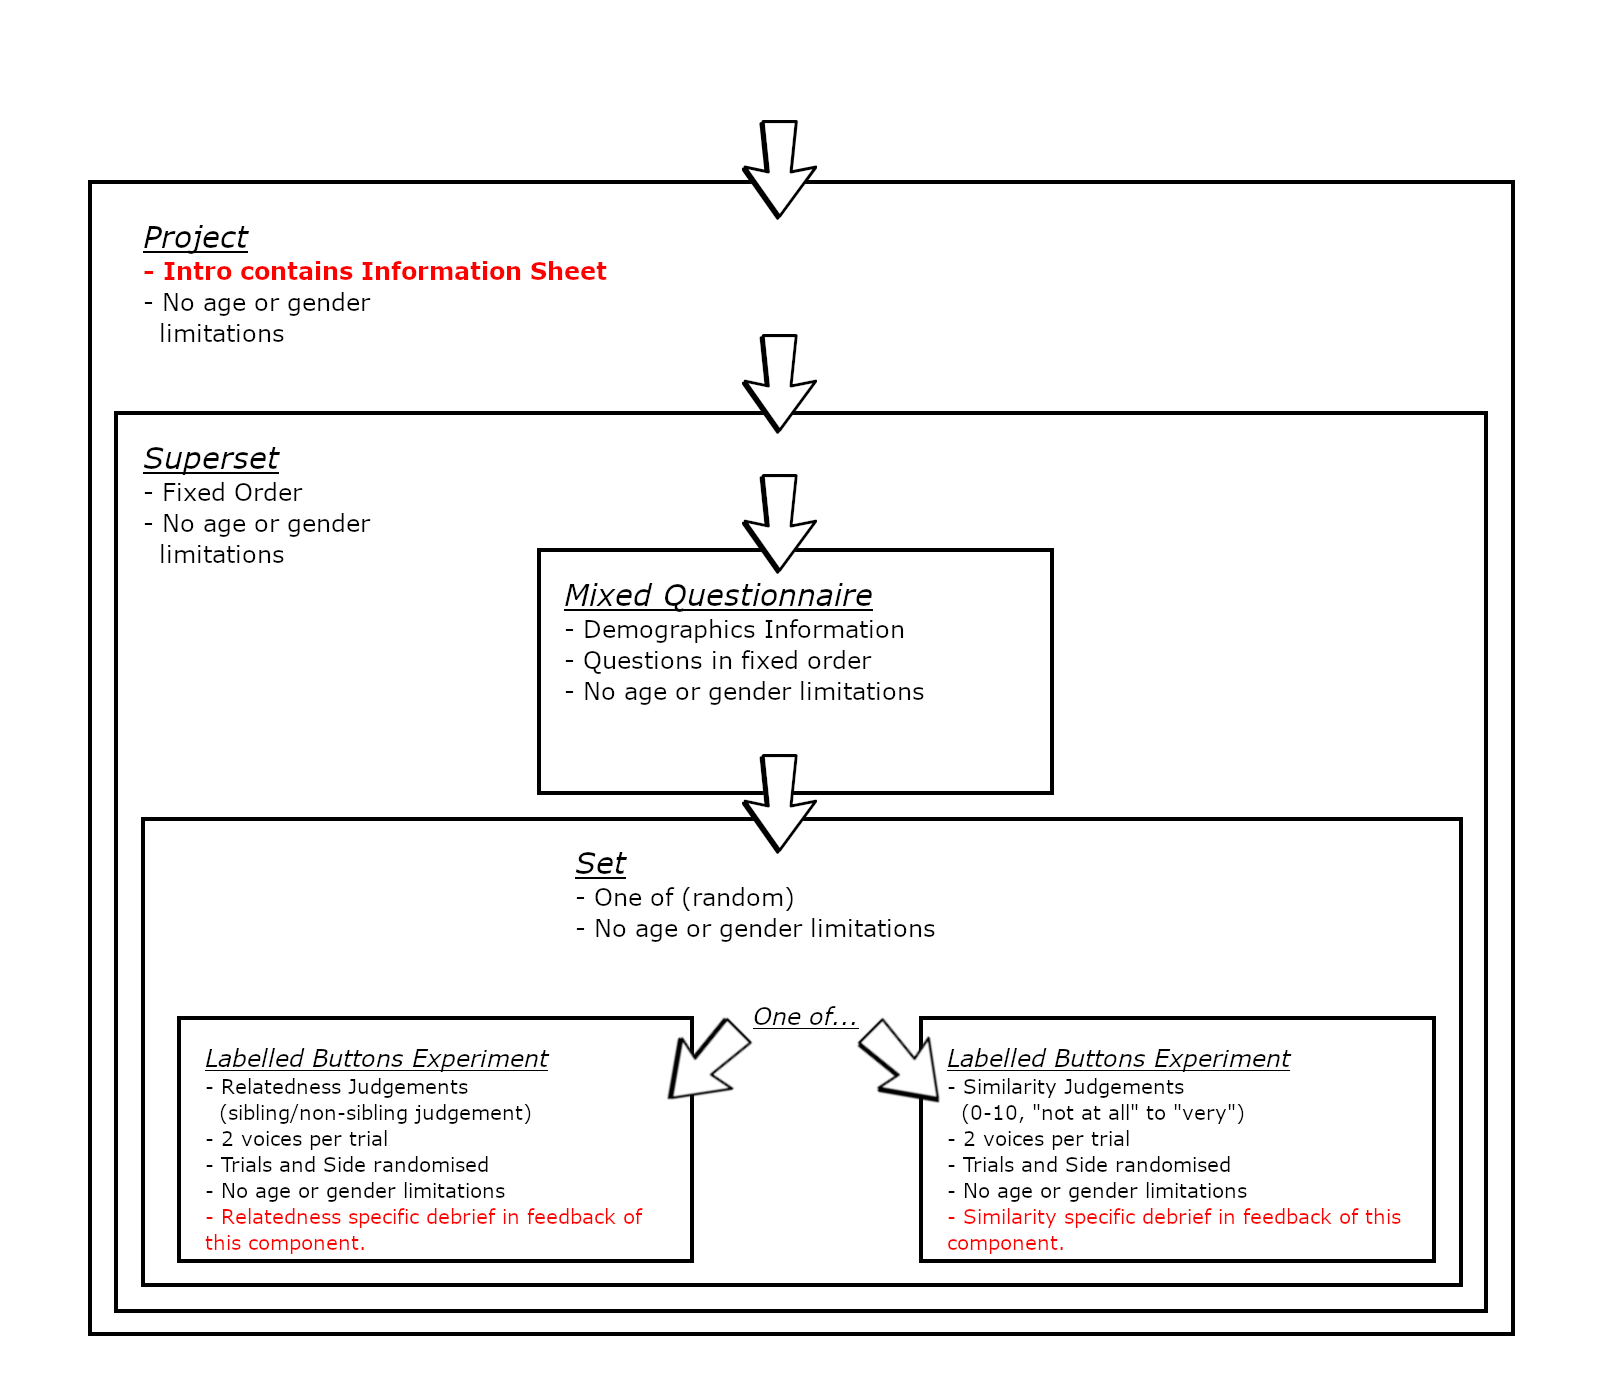
\includegraphics{images/screenshots/structure.png}

This will be displayed to the participants after they have completed the
component or components (depending on your design) in the superset. You
can see the feedback displayed in a
\protect\hyperlink{sample_order}{sample order}:

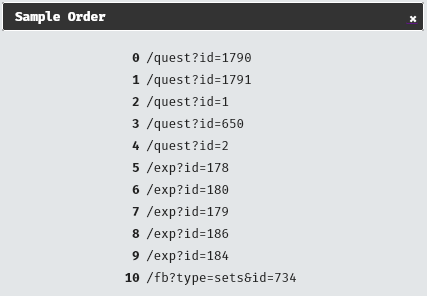
\includegraphics{images/screenshots/sets_14.png}

The debriefing information should be placed in the General Feedback
section on the set information, as shown below:

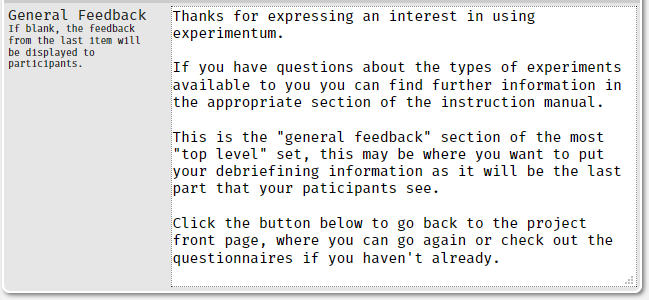
\includegraphics{images/screenshots/feedback.png}

The General Feedback section can be formatted using Markdown or HTML
tags. If you use HTML tags, ensure that your opening and closing tags
are matched to prevent errors.

\chapter{Questionnaire Components}\label{questionnaire-components}

\section{Overview}\label{overview-3}

Questionnaires are currently the most used items on Experimentum. They
are made up of one or more individual components, available in 3
different types: mixed, radiopage and ranking.

\section{New Questionnaire}\label{new-questionnaire}

To create a new questionnaire, navigate to the researcher's section of
the page by using the menu on the right and selecting the questionnaires
option.


\includegraphics{images/screenshots/questionnaire_button.png}

From here, you will be able to see the questionnaires for which you have
ownership status (ones you have created yourself, or ones that someone
else has shared with you). To create a new questionnaire, click the
button on the top right ``New Questionnaire'':

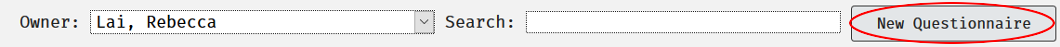
\includegraphics{images/screenshots/new_questionnaire.png}

The following pop-up box will appear, allowing you to choose the type
that you want to create:

\includegraphics{images/screenshots/questionnaire_dialogue.png}

The types that you choose will depend on what type of functionality your
study requires. You should note that pencil and paper questionnaires
will not always be able to be copied exactly onto Experimentum. If you
make any changes to questionnaires to deliver them electronically you
should discuss required changes with your supervisor to ensure their
validity has not been compromised.

\section{Save Questionnaire and Reset
Buttons}\label{save-questionnaire-and-reset-buttons}

Once you have entered information about the questionnaire you should
save it. Saving regularly is good practice. Do this by pressing the save
questionnaire button.

The reset button is akin to a ``revert'' button, where any changes made
after the last save can be discarded and you return to the last saved
version.

\begin{danger}
The JavaScript for saving the questionnaire occasionally stops working
on some browsers, so we recommend saving the questionnaire after every 3
or so changes to minimise loss of work in the event of an error.

Please note that the site currently does not support version control, so
once you save a change the previous version will be overwritten.
\end{danger}

\section{Questionnaire Information}\label{questionnaire-information}

All types of questionnaires will ask you to provide information about
it, the only difference will be the Questionnaire Type, which will
correspond to the type of questionnaire you have chosen on the previous
pop-up box.

\includegraphics{images/screenshots/quest_info.png}

\begin{itemize}
\tightlist
\item
  \textbf{Name for Users}: this is the name of this component that will
  be displayed to users. Please ensure that it is appropriate.
\item
  \textbf{Name for Researchers}: this is the name of this component for
  researchers. It will be displayed on lists and visible to you, your
  supervisor and admin staff. It should be informative and appropriate.
\item
  \textbf{Question Order}: this indicates how you want Experimentum to
  display the questions contained \textbf{in this component only}.

  \begin{itemize}
  \tightlist
  \item
    Fixed will display the questions to the participants in the order
    you have put them on this page.
  \item
    Random will mix the order of question presentation up automatically.
    Order of presentation will be recorded in your data when you
    download it.
  \end{itemize}
\item
  \textbf{Limited to}: limitations will only allow people in a certain
  age range and with a certain gender identity to complete this
  component of the study.

  \begin{itemize}
  \tightlist
  \item
    If you are planning on allowing anonymous participation you should
    not set limitations as age and gender identity of these users will
    be unknown and may not be allowed to do these sections of the study
    if participants refuse this information.
  \end{itemize}
\item
  \textbf{Labnotes}: this is a short blurb about this component of your
  study. You should always add lab notes so that you, your supervisor
  and the admins will be able to tell what this component is about. The
  following sections will describe each questionnaire type and what they
  can do.
\end{itemize}

\section{Questionnaire Tab}\label{questionnaire-tab}

The questionnaire tab on the lower half of the page is different for
each questionnaire. Please see the appropriate sections below for more
information on these.

\section{Feedback Tab}\label{feedback-tab}

In most cases you should leave this empty. The feedback for the top-most
set is normally where you would put your debriefing information. You can
see the later sections on projects and debriefing.

\section{Adding/Deleting Questions}\label{addingdeleting-questions}

\begin{warning}
All questions \textbf{must} be given unique names within the component
they are in. Components cannot be saved if you have questions with
duplicate names.

This applies to questions added individually or in bulk.

You might find it easier to give each question across the entire study
unique names.
\end{warning}

\subsection{Adding Individually}\label{adding-individually}

In order to add a new question, you must ensure that all editing options
are closed on the existing questions by clicking the pencil to get rid
of the yellow surround or the cog to close the menu.

Pressing the button at the bottom of the page will allow you to add a
new question.

Experimentum will add a new question by directly duplicating the
previous question, with all the same text and attributes. Please ensure
that you set a unique name for the new question before you attempt to
save the questionnaire as questions with duplicate names will be removed
by the system.

\begin{danger}
The JavaScript for saving the questionnaire occasionally stops working
on some browsers, so we recommend saving the questionnaire after every 3
or so changes to minimise loss of work in the event of an error.
\end{danger}

\hypertarget{addfromspreadsheet}{\subsection{Adding in
Bulk}\label{addfromspreadsheet}}

It is also possible to add some types of questions in bulk by using a
spreadsheet. Unfortunately, not all types are covered, but the most
basic and most frequently used types are. Spreadsheet templates are
available by clicking ``add from spreadsheet'' and selecting the
underlined type of questionnaire from the options just above the
buttons.

\includegraphics{images/screenshots/quest_spread_1.png}

Each of the column headers will relate to each of the question
attributes you would use when setting the questions manually. For
ranking and radiopage questionnaires not all of these headers will be
applicable. Double click on the ones you do not need to remove them as I
have done in the image below:

\includegraphics{images/screenshots/quest_spread_2.png}

Fill the template spreadsheet in and save it onto your own storage, copy
the cells that contain your question information. See the section below
for more about question information. Double click on the section that
says, ``Double-click to paste data from a spreadsheet'' and paste it
when in the new entry box that appears:

\includegraphics{images/screenshots/quest_spread_3.png}

If you do not use the template spreadsheet, but one you have made
yourself, ensure that the options that you are specifying match. You can
also drag the headers on the entry window from left to right to re-order
them if your own spreadsheet does not match the headers here.

\begin{tabular}{l|l|l}
\hline
Column Header: & Refers to: & Options:\\
\hline
name & dv\_name (in data = q\_name) & Names must only contain letters, underscores and numbers (numbers must not be the first characters).\\
\hline
question & The question that you are asking the participant. & Whatever you want to ask the participant.\\
\hline
type & The type of question, akin to the options selected from the menu opened by the cog & * select: pulldown menu \textbackslash{}n* selectnum: numeric pulldown menu \textbackslash{}n* radio: radiobuttons \textbackslash{}n* radioanchor: radiobuttons with anchors \textbackslash{}n* datemenu: date menu \textbackslash{}n* text: short text\\
\hline
options & Where you would specify the response options available to the participants. & Applicable to select and radio types. \textbackslash{}n*  Numerical code, followed by ":", and then text option. \textbackslash{}n*  Specifying multiple by separating options using a semi-colon (;)\\
\hline
maxlength & Where you would specify the length of the response & Applicable to radioanchor and text. \textbackslash{}n*  Radioanchor: how many points in the range. \textbackslash{}n*  Text: how many characters allowed.\\
\hline
low\_anchor & Specifying the low anchor for the selected option. & Applicable to selectnum, radioanchor and datemenu. \textbackslash{}n*  Selectnum specifies the lowest number in the range of the dropdown menu \textbackslash{}n*  Radioanchor specifies the text for low anchor \textbackslash{}n*  Datemenu specified the lower end of the year range.\\
\hline
high\_anchor & Specifying the high anchor for the selected option. & Applicable to selectnum, radioanchor and datemenu. \textbackslash{}n*  Selectnum specifies the highest number in the range of the dropdown menu\textbackslash{}n*  Radioanchor specifies the text for high anchor\textbackslash{}n*  Datemenu specified the higher end of the year range.\\
\hline
\end{tabular}

Each of the three types of questionnaire component has their own
template spreadsheet available for download, which are linked in the
dialogue box you get when you click to ``add from spreadsheet''. If you
intend to add questions in bulk you should consult these spreadsheets
for guidance in the first instance as examples are given.

\subsection{Re-Order Questions}\label{re-order-questions}

If you wish to present your questions in a specific order, and this
order is different than what you have in your questionnaire component,
you can click on the arrows button between the dv\_name and the question
text to move the question up or down the order of presentation.

\includegraphics{images/screenshots/qreorder.png}

\subsection{Deleting Questions}\label{deleting-questions}

Questions can be erased by clicking the picture of the trash/bin next to
the question you want to delete.

\includegraphics{images/screenshots/bin.png}

\begin{danger}
Please note that the site currently does not support version control, so
once you save a change the previous version will be overwritten. This
includes deleted questions- once you have saved the changes they are
gone.
\end{danger}

\section{Questionnaire Types}\label{questionnaire-types}

\subsection{Mixed Questionnaire}\label{mixed-questionnaire}

Allows you to present multiple question types and gather multiple
response types in a single component. When you select a mixed
questionnaire, you will be taken to this page:

\includegraphics{images/screenshots/quest_mixed.png}

As you can see you have the same questionnaire information section at
the top, as you will have in all questionnaires. The differences lie in
the types of questions that you can include. Mixed questionnaires can
accommodate multiple types of questions on a single page.

\subsubsection*{Attributes}\label{attributes}
\addcontentsline{toc}{subsubsection}{Attributes}

\begin{itemize}
\tightlist
\item
  \textbf{Instructions}: when you click the part that says ``Click here
  to set instructions'' you will be able to enter text instructions to
  the participants for this entire component. You will also be able to
  enter Markdown and HTML code, which allows you to link to and embed
  additional media or format the text in specific ways.

  \begin{itemize}
  \tightlist
  \item
    If you use HTML tags you must ensure that you have matching opening
    and closing tags, as unmatched ones will prevent the component from
    recording data.
  \end{itemize}
\item
  \textbf{dv\_name}: this is the name of the dependent variable, the
  name that will be assigned to the column q\_name in the downloaded
  data indicating which question the participant has answered. You
  should set one which is unique to this component and perhaps across
  all components.

  \includegraphics{images/screenshots/qname.png}
\item
  \textbf{Question}: clicking the part which says ``click here to set
  your question'' will allow you to enter the question text that the
  participants will see, the question that you want to ask them.

  \includegraphics{images/screenshots/qtext.png}
\end{itemize}

\subsubsection*{Changing Question and Response
Type}\label{changing-question-and-response-type}
\addcontentsline{toc}{subsubsection}{Changing Question and Response
Type}

Clicking the cog next to the question and then the arrow in the
resulting menu will allow you to choose the type of question you want to
set.

\includegraphics{images/screenshots/quest_mixed_1.png}

When you have selected the type of question, you can then edit the
response types that can be made by the participants by clicking the
pencil next to the cog. When this editing mode is active, the response
section will be unfolded, and will be displayed with a yellow surround.

\includegraphics{images/screenshots/quest_mixed_2.png}

\begin{warning}
You must close this editing mode by clicking the pencil a second time,
getting rid of the yellow surround, \textbf{before} you add a new
question, click the cog or save the questionnaire.
\end{warning}

\subsubsection*{Question Types}\label{question-types}
\addcontentsline{toc}{subsubsection}{Question Types}

\begin{itemize}
\tightlist
\item
  \textbf{Pulldown Menu}: pulldown menus give your participants a set of
  text option responses to choose from. Each text option has a numeric
  coding value associated with it, which will be the returned value in
  the downloaded data in place of the text. This is specified before the
  colon. The text options are specified after the colon, these are not
  returned in the data.

  \includegraphics{images/screenshots/quest_mixed_3.png}

  \begin{itemize}
  \tightlist
  \item
    Each text value should be associated with a unique numerical coding
    value, non-unique numerical codes will be deleted upon saving the
    questionnaire. You can add multiple options to the menu.
  \end{itemize}
\item
  \textbf{Numeric Pulldown Menu}: this allows you to set numerical
  values to a pulldown menu, with no associated text label. The range
  that is set is the range that will be displayed to the user, as below.

  \begin{itemize}
  \tightlist
  \item
    You should use whole numbers only.

    \includegraphics{images/screenshots/quest_mixed_4.png}

    \includegraphics{images/screenshots/quest_mixed_5.png}
  \end{itemize}
\item
  \textbf{Slider}: sliders provide you with a way for participants to
  return a finer-grained numerical response on a spectrum between two
  anchor points. A slider scale will be displayed to participants, with
  the low end of the range associated with the low anchor, and the high
  end the high anchor. Participants will move a slider along the scale,
  and a numerical value associated with the position they put it in
  returned in the data. You set the scale limits and increments, in this
  example from 0 to 100 in increments of 1.

  \begin{itemize}
  \tightlist
  \item
    You can also change the text anchors by clicking on them as shown
    here.

    \includegraphics{images/screenshots/quest_mixed_6.png}
  \item
    Slider knobs do not appear until the participant has clicked
    somewhere on the scale.
  \end{itemize}
\item
  \textbf{Radio Buttons with Anchors}: this option allows you to set a
  scale with a low anchor and a high anchor, which you can change by
  clicking the text. You can add or remove points to the scale by
  pressing the + and -- buttons on either side of the response. On this
  scale example below, a number will be returned associated with the
  point on the scale the participant submitted, here 1 (lowest) to 5
  (highest).

  \includegraphics{images/screenshots/quest_mixed_7.png}
\item
  \textbf{Date Menu}: date menus allow the participants to choose a
  specific date. You can set the range of dates to choose from, in the
  example below the participant is allowed to go back 100 years from the
  current date (-100y) but cannot go further into the future than today
  (+0y). When participants click on the response, they will be given a
  calendar to pick from, instead of typing the date.

  \includegraphics{images/screenshots/quest_mixed_8.png}

  \includegraphics{images/screenshots/quest_mixed_9.png}
\item
  \textbf{Time}: This allows participants to enter a time, in 24 hour
  format, using hours and minutes.

  \includegraphics{images/screenshots/quest_mixed_14.png}

  \includegraphics{images/screenshots/quest_mixed_15.png}

  You can change the response options (from single minutes to increments
  of 15, for example), but it is not advised.
\item
  \textbf{Countries}: participants can choose from a list countries.
  Returned in the data as the two letter ISO-3166-1 alpha-2 code.

  \includegraphics{images/screenshots/quest_mixed_10.png}
\item
  \textbf{Short Text}: allows participants to enter free-response text
  up to and including 255 characters. Returned in the data as character
  strings. The maximum number of characters can be changed by changing
  the number after \texttt{maxlength:}.

  \includegraphics{images/screenshots/quest_mixed_11.png}
\item
  \textbf{Long Text}: allows participants to enter free-response text
  over 255 characters. Returned in the data as character strings. If you
  do not need more than 255 characters, please use the short text to
  minimise strain on the server.

  \includegraphics{images/screenshots/quest_mixed_12.png}
\item
  \textbf{Message}: allows you to put a line of text into a
  questionnaire which does not require a response amongst other
  questions. Note that to ensure that this appears where it should that
  these questions should be presented in a fixed order.

  \includegraphics{images/screenshots/quest_mixed_13.png}
\end{itemize}

\subsection{Radiopage}\label{radiopage}

Radiopage questionnaires contain the same questionnaire information
section at the top of the page as a Mixed Questionnaire.

The format of this questionnaire allows the user to set a number of
questions with radio button responses on a single page, with a single
response scale for all questions.

Each point on the scale has its own text label, and an ``option value''
number associated with it, rather than only the two extremities of a
multiple point scale as in the radio buttons with anchors in the mixed
questionnaire.

\includegraphics{images/screenshots/radio_1.png}

\subsubsection*{Attributes}\label{attributes-1}
\addcontentsline{toc}{subsubsection}{Attributes}

\begin{itemize}
\tightlist
\item
  \textbf{Instructions}: when you click the part that says ``Click here
  to set instructions'' you will be able to enter text instructions to
  the participants for this entire component. You will also be able to
  enter Markdown and HTML code, which allows you to link to and embed
  additional media or format the text in specific ways. See
  \protect\hyperlink{htmlstim}{stimuli} for more information on this.
\item
  \textbf{Option values}: these are the numerical equivalents of the
  text labels for each of the responses a participant can make to any
  question on the page. This number is not displayed to participants.
  The number you set is largely arbitrary, but the numerical figure
  associates with the choice rendered by participants is returned in the
  data set upon download and text values are not. You will need to know
  what number corresponds to which text response in order to carry out
  and interpret your analyses. It is possible to have automatic reverse
  scoring- see \protect\hyperlink{fwdrev}{here} for more information.
\item
  \textbf{Option text}: this is the text label associated with each
  response the participant can make to any question on the page. The
  associated text is what the participant sees, and it is displayed in
  the construction page directly below the numerical value you set. The
  option text is not returned in the downloaded data set.
\item
  \textbf{Adding/removing options}: you can add or remove the number of
  response options on the scale you give to participants by pressing the
  + or -- symbols in circles on the right of the scale at the top of the
  questionnaire.
\end{itemize}

\includegraphics{images/screenshots/radio_2.png}

\begin{itemize}
\tightlist
\item
  \textbf{dv\_name}: this is the name of the dependent variable, the
  name that will be assigned to the column q\_name in the downloaded
  data indicating which question the participant has answered. You
  should set one which is unique within this component, or perhaps
  across all components in your study.

  \includegraphics{images/screenshots/qname.png}
\item
  \textbf{Question}: clicking the part which says ``click here to set
  your question'' will allow you to enter the question text that the
  participants will see, the question that you want to ask them.

  \includegraphics{images/screenshots/qtext.png}
\end{itemize}

\hypertarget{fwdrev}{\subsubsection*{Forward and Reverse
Scoring}\label{fwdrev}}
\addcontentsline{toc}{subsubsection}{Forward and Reverse Scoring}

In many questionnaires it is common to find items which should be
``reverse-scored''. Here you can indicate if the question is forward or
reverse scored, and the system will make the changes to the data for
you, saving you from having to recode them later.

Example: your scale at the top indicates 1-5 as below. As you can see
``much less than average'' is associated option value of 1. The forward
scored question is marked ``fwd'' in the pulldown menu on the right of
the table and the reverse scored question is marked ``rev''.

\includegraphics{images/screenshots/radio_3.png}

If a participant chooses ``much less than average'' on a forward scored
question the dv in the output will be ``1''. But what happens to the
reverse scored question?

\includegraphics{images/screenshots/radio_4.png}

This is the data output here. As you can see where the participant chose
the option that returned a ``1'' for the forward scored question, for
the reverse scored question that same choice returns a ``5'' in the
data.

\includegraphics{images/screenshots/radio_5.png}

\subsection{Rank Order}\label{rank-order}

Ranking questionnaires present a list of text options to participants to
put into a specific order, based on some judgement they are asked to
make on them.

\includegraphics{images/screenshots/rank1.png}

As you can see, there are no response types associated with this
questionnaire type. The DV in this case will be the rank position
assigned by the participants. Setting the order to fixed will set the
initial order up on the order you have specified on the questionnaire
editing page and random will randomise it.

Each question will be an option in the list of items to rank order.
Participants will be able to drag each text item to rank order them,
with the number specified in the column next to the text. The final
presentation to participants looks like this:

\includegraphics{images/screenshots/rank2a.png}

\includegraphics{images/screenshots/rank2b.png}

\includegraphics{images/screenshots/rank2c.png}

In the data, the question name is saved as q\_name and the rank order
assigned by the participant is saved as the dv in the downloaded data:

\includegraphics{images/screenshots/rank3.png}

\hypertarget{assignstimquest}{\section{Using Stimuli with
Questionnaires}\label{assignstimquest}}

In some cases you might wish to include some stimuli with a
questionnaire. For example, you might want to present an image with a
set of questions asking the user's opinions about that image.

We would recommend that you upload your image as per the instructions
given in the \protect\hyperlink{stimuli}{stimuli} page and use HTML or
Markdown in the instructions at the top of the questionnaire component
that you want to display the stimuli on.

First, you will need to find the path of the stimuli you have uploaded
to the server by going to ``My Uploaded Stimuli'' by navigating to
Researchers\textgreater{}Stimuli\textgreater{}Upload Stimuli and looking
in the folders at the bottom of the page. Find the image that you want
to use and click on it in the folders. It will display on the right hand
side and the file path will be above it. Copy the file path, seen
circled here:

\includegraphics{images/screenshots/quest_stim_1.png}

Next you will need to paste that into the introduction box using an
appropriate image tag. Here you can see the HTML syntax to link to an
image:

\includegraphics{images/screenshots/quest_stim_2.png}

The code is:

\begin{Shaded}
\begin{Highlighting}[]
\OperatorTok{<}\NormalTok{center}\OperatorTok{>}\ErrorTok{<}\NormalTok{img src=}\StringTok{"file/path/here.jpg"}\NormalTok{ width=}\StringTok{"500px"}\OperatorTok{>}\ErrorTok{</}\NormalTok{center}\OperatorTok{>}
\end{Highlighting}
\end{Shaded}

\texttt{width=500px} alters the image displayed by resizing the image to
be 500 pixels wide whilst maintaining the aspect ratio.

This is OK for one or two images, but if you are doing this with many
images we would recommend that you resize the stimuli before uploading
them.

\texttt{\textless{}center\textgreater{}} ensures that the image stays in
the middle of the page. \texttt{\textless{}/center\textgreater{}} is a
``closing tag'' and must be put in place to ensure that data for the
component is saved to the server.

When participants go through the questionnaire this is what they will
see:

\includegraphics{images/screenshots/quest_stim_3.png}

This method works for all types of compatible stimuli, although the code
used to display them will vary.

For audio:

\begin{Shaded}
\begin{Highlighting}[]
\OperatorTok{<}\NormalTok{center}\OperatorTok{>}\ErrorTok{<}\NormalTok{audio controls}\OperatorTok{>}
\StringTok{  }\ErrorTok{<}\NormalTok{source src=}\StringTok{"file/path/here.mp3"}\NormalTok{ type=}\StringTok{"audio/mpeg"}\OperatorTok{>}
\NormalTok{Your browser does not support the audio element.}
\OperatorTok{<}\ErrorTok{/}\NormalTok{audio}\OperatorTok{>}\ErrorTok{</}\NormalTok{center}\OperatorTok{>}\StringTok{ }
\end{Highlighting}
\end{Shaded}

Displayed as a small media player:

\includegraphics{images/screenshots/quest_stim_4.png}

And for video:

\begin{Shaded}
\begin{Highlighting}[]
\OperatorTok{<}\NormalTok{center}\OperatorTok{>}\ErrorTok{<}\NormalTok{video width=}\StringTok{"320"}\NormalTok{ height=}\StringTok{"240"}\NormalTok{ controls}\OperatorTok{>}
\StringTok{  }\ErrorTok{<}\NormalTok{source src=}\StringTok{"file/path/here.m4v"}\NormalTok{ type=}\StringTok{"video/mp4"}\OperatorTok{>}
\NormalTok{Your browser does not support the video tag.}
\OperatorTok{<}\ErrorTok{/}\NormalTok{video}\OperatorTok{>}\ErrorTok{</}\NormalTok{center}\OperatorTok{>}
\end{Highlighting}
\end{Shaded}

\begin{info}
Whilst you \emph{can} link to externally hosted stimuli we would
recommend that \textbf{if possible} you upload your stimuli to our
server. This will ensure uninterrupted access to your media.

We cannot always host all stimuli. Files larger than 3mb each should be
uploaded elsewhere to suitable platforms, such as YouTube, as loading
times are often too long for files which exceed this limit.

Embedding media from outside sources may require different code than
provided above.
\end{info}

See the \protect\hyperlink{stimuli}{stimuli} page for further
information on preprocessing and uploading stimuli.

\chapter{Experimental Components}\label{experimental-components}

\section{Overview}\label{overview-4}

Simple behavioural experiments can also be run through Experimentum,
using a variety of different stimuli media and with a wide selection of
design choices that can be combined. To create a new experiment
component, navigate to the ``researchers'' section by using the menu on
the right side of the page.

This is an overview of the types of experimental components avaible to
you:

\begin{tabular}{l|l|l}
\hline
Experiment Type & Response Type & DV\\
\hline
2AFC & Alternative force choice with 2 options to choose from & Binary, defaulted to 0 or 1 assigned depending on how you assign the stimuli to trials.\\
\hline
2-AFC with 8 button strength of choice & Alternative force choice between two stimuli, but with the addition of strength of preference for the choice made on an 8-point scale. & Out of 8, with 0-3 indicating strength of choice in one direction for one piece of stimuli and 4-7 indicating strength of choice in the other direction for the other piece of stimuli.\\
\hline
Labelled Buttons & Display 1, 2 or 3 stimuli items and participants respond on a scale set by the researcher. Akin to a Likert scale. & A numerical value corresponding to the values set by the researcher.\\
\hline
Slider & A sliding scale between two numerical points where the number is not displayed to participants. & Numerical, between upper and lower bounds and at increments set by the researcher.\\
\hline
X-AFC & Alternative forced choice with more than 2 options. Participants pick only one. & DV is a number which corresponds to the column the chosen stimuli item is assigned to on the stimuli assignment page, ranging from 1 to X.\\
\hline
Sorting & Participants put stimuli in order of some specified preference by dragging them into position on the screen & Number of times participants changed the order and the order the stimuli was placed in. Also provides stimuli original order of presentation.\\
\hline
Slideshow & Timed display of stimuli items where participants are only asked to watch, with no data collected or rendered. Usually used as a precursor to another component. & None.\\
\hline
\end{tabular}

These will be covered in further detail in the section on
\protect\hyperlink{exp_types}{experimental component types}.

Some types require specific considerations in the interpretation of the
data, assignment of stimuli, etc. Please read the one(s) that concern
you carefully.

You are also given a look at the view the participants will see in an
individual trial for each type.

\section{Creating a New Component}\label{creating-a-new-component}

Click on the ``New experiment'' button at the top of the page to create
a new experiment, and select the type of experiment that you want to
make from the dialogue box:

\includegraphics{images/screenshots/exp_1.png}

\includegraphics{images/screenshots/exp_2.png}

This displays all of currently available experimental component types
available for you to use.

\subsection{Experiment Information}\label{experiment-information}

All experiment types have a generic information fields in common, but
some have extra depending on their functionality. Each of the options
common across all types of experiment will be discussed in the following
section. Where information is specific to a certain type of experiment
it will be specified in brackets what type of experiment it refers to.

You should make your information section as detailed as possible to
remind your future self of what you have done, but also to explain what
you have done to your supervisor(s) and the admins who will use this
information to provide support. Here is an information section from a
2-AFC questionnaire for reference:

\includegraphics{images/screenshots/exp_6.png}

\begin{itemize}
\item
  \textbf{Name for Users}: this is the name of this component that will
  be displayed to users. Please ensure that it is suitable.
\item
  \textbf{Name for Researchers}: this is the name of this component for
  researchers. It will be displayed on lists and visible to you, your
  supervisor and admin staff. It should be informative and appropriate.
\item
  \textbf{Design}: within or between subjects, allow for multiple
  completions or single completion only.
\item
  \textbf{Slider range}: (slider only). This determines the numerical
  value associated with each position on the slider, and the increments
  along it.
\item
  \textbf{Trial Order}: this indicates how you want Experimentum to
  display the individual trials contained in this component only. Fixed
  will display the trials in the order set on the ``edit trials''
  section later. Random will mix the order of question presentation up
  automatically. Order of presentation will be recorded in your data
  when you download it.
\item
  \textbf{Image side}: (2-AFC, 2-AFC with 8 button strength of choice
  only). Fixed will display images on the side specified in the ``edit
  trials'' section later. Random will switch the side of presentation
  randomly. Side of presentation will be recorded in your data.
\item
  \textbf{Images}: allows you to present a subset of your stimuli to
  your participants. For example, if you have 40 pairs of faces from
  which to choose the more trustworthy, you can present a subset of 20
  pairs of faces to each participant by setting this to ``Show 20 of 40
  total images''.
\item
  \textbf{Limited to}: limitations will only allow people in a certain
  age range and with a certain gender identity to complete this
  component of the study. If you are planning on allowing anonymous
  participation you should not set limitations as age and gender
  identity of these users will be unknown, and they will not be allowed
  to do these sections of the study if they refuse to submit this
  information.
\item
  \textbf{Labnotes}: this is a short blurb about this component of your
  study. You should always add lab notes so that you, your supervisor
  and the admins will be able to tell what this component is about.
\item
  \textbf{Number of images to display}: this specifies the number of
  images to display per trial. You may wish to display 1, 2 or more
  depending on your design.
\end{itemize}

\subsubsection{Experiment info: what are these
tabs?}\label{experiment-info-what-are-these-tabs}

All experiment components will present you with 3 tabs under the
experiment information section. The following section discusses when the
participants will see them, and make suggestions on how you may want to
use these.

\paragraph{Introduction Tab}\label{introduction-tab}
\addcontentsline{toc}{paragraph}{Introduction Tab}

Before each component starts to run participants will be greeted with a
short introduction to the component. You should include some
instructions to the participants here. Here is an example from the 2 AFC
type of experiment:

\includegraphics{images/screenshots/exp_7.png}

The text above will appear to the participants immediately prior to the
start of the first trial:

\includegraphics{images/screenshots/exp_8.png}

This text can be formatted with HTML or Markdown code. If you use HTML
tags you must ensure that you have matching opening and closing tags, as
unmatched ones will prevent the component from recording data.

\paragraph{Experiment Tab}\label{experiment-tab}
\addcontentsline{toc}{paragraph}{Experiment Tab}

Once you have written your instructions to your participants, click on
the experiment tab next to introduction. Set the question here if the
question is to remain the same across all trials within this component.

\includegraphics{images/screenshots/exp_9.png}

If you choose to leave the question blank, delete the question and
``\{\{blank\}\}'' will be displayed above the stimuli images on this
tab, and will be empty on each trial displayed to participants. If you
wish to have the question vary by trial, you should leave the question
blank. When you come to assign stimuli to trials you can type in
questions according to which trial is being displayed.

If your experiment uses a scale with anchor points or text labels for
buttons, you would click them to edit in the same way as the questions.
Here is an example from the Slider type experiment, where there are
anchors at the left and right most extremes of the scale:

\includegraphics{images/screenshots/exp_10.png}

An example of changing participant-facing button labels in a labelled
button experiment:

\includegraphics{images/screenshots/exp_11.png}

Check that the number of stimuli displayed on this page are correct.
Here, the ``blankface'' image is displayed as a placeholder for your own
stimuli, regardless of the type of stimuli you are placing/have already
placed. Then check that the number of trials is correct at the bottom of
the page too.

\paragraph{Feedback Tab}\label{feedback-tab-1}
\addcontentsline{toc}{paragraph}{Feedback Tab}

Generally, the feedback tab in individual components should be left
alone. This will be covered later in the section covering Debriefing.

\section{Saving your Component}\label{saving-your-component}

Saving experiments differs slightly from saving questionnaires. When you
save an experiment, you will be taken to the trial editing page (see
individual experiment types on how to fill in your stimuli). The reset
button remains the same, it will revert to the last saved version of the
experiment:

\includegraphics{images/screenshots/exp_3.png}

\section{Accessing and Editing Previously Saved
Experiments}\label{accessing-and-editing-previously-saved-experiments}

To access your previously saved experiment component, navigate to the
researcher's area of the site by selecting ``Researchers'' from the menu
on the right-hand side of the page.

You can access your experiments by accessing the experiments section of
the page by using the button below:

\includegraphics{images/screenshots/exp_4.png}

Alternatively, if you remember the number of the experiment component,
you can type it in to the grey rectangle in the experiments button. When
you press return you will be taken straight to the information page of
the experiment.

To edit the experiment, press the ``edit'' button at the top of the page
and you will be taken back into the editable version:

\includegraphics{images/screenshots/exp_5.png}

\begin{warning}
If you edit and save changes to a component which is currently active
you will deactivate it.

If you are a student researcher this will mean you will need to contact
your supervisor again to re-activate it.
\end{warning}

\hypertarget{exp_types}{\section{Types of Components}\label{exp_types}}

There are different types of experimental components for you to choose
from. They each have their own features, response types and type of DV
that they return in your data. The following section will discuss each
of the options available to you.

\subsection{2-AFC (alternative forced
choice)}\label{afc-alternative-forced-choice}

2-AFC experiments present participants with 2 options and ask them to
make a choice between them. Here you will present 2 stimuli items
together and ask participants to make a binary judgment between the two
by clicking on one item only. The DV returned will be either a 1 or a 0,
depending on the choice the participant makes and what stimuli item you
define as a 1 or a 0 when you assign stimuli to trials (see
\protect\hyperlink{twoafc_notes}{Notes specific to 2-AFC} below).

Open a new experiment by clicking the ``new experiment'' button on the
researcher's page and select 2-AFC from the dialogue box:

\includegraphics{images/screenshots/exp_1.png}

\includegraphics{images/screenshots/exp_2.png}

First, you should complete the experiment information at the top of the
page, then set instructions on the introduction tab. For example, I have
12 pairs of faces in my Mooney faces set that I uploaded in the
\protect\hyperlink{stimupload}{uploading stimuli} section, so I would
change the number of total images to 12.

Once you have finished on this page and press ``Save'' you will be taken
to the page that allows you to assign stimuli , assign trial names and
(if applicable) individual questions for the trials.

\hypertarget{twoafc_notes}{\subsubsection*{Notes Specific to
2-AFC}\label{twoafc_notes}}
\addcontentsline{toc}{subsubsection}{Notes Specific to 2-AFC}

When you assign stimuli to the 2-AFC be sure that you assign the correct
stimuli according to the DV that you expect to be returned.

In the screenshot below you can see that one column corresponds to a DV
of 1 and the other a DV of 0. Ensure that you assign the stimuli you
wish to return a DV of 1 and the stimuli you wish to return a DV of 0 to
the appropriate columns.

\includegraphics{images/screenshots/stim_2afc.png}

\subsubsection*{Participant View}\label{participant-view}
\addcontentsline{toc}{subsubsection}{Participant View}

When this experimental component is presented to the participants it
will look like this:

\includegraphics{images/screenshots/view_2afc.png}

\subsection{2-AFC with 8-Button Strength of Choice
(JND)}\label{afc-with-8-button-strength-of-choice-jnd}

For the most part, the 2-AFC with 8 button strength of choice is largely
the same as the binary 2-ACF experiment type in its presentation, but
the question being asked and the DV rendered by participants differ.

You will still be asking participants to compare the two stimuli pieces
and render a judgement. Instead of asking them to pick one, you will be
asking them to pick one \emph{and} indicate the strength of their
choice. This type is also referred to as the large\_n JND type in the
component information page.

\includegraphics{images/screenshots/jnd.png}

Open a new experiment by clicking the ``new experiment'' button on the
researchers' page and select 2-AFC with 8-button strength of choice from
the dialogue box:

\includegraphics{images/screenshots/exp_2.png}

First, you should complete the experiment information at the top of the
page, then set instructions on the introduction tab. For example, I have
12 pairs of faces in my Mooney faces set that I uploaded earlier in the
uploading stimuli section, so I would change the number of total images
to 12.

Once you have finished on this page and press ``Save'' you will be taken
to the page that allows you to assign stimuli , assign trial names and
(if applicable) individual questions for the trials.

\subsubsection*{Notes Specific to 2-AFC with 8-Button Strength of
Choice}\label{notes-specific-to-2-afc-with-8-button-strength-of-choice}
\addcontentsline{toc}{subsubsection}{Notes Specific to 2-AFC with
8-Button Strength of Choice}

\paragraph{Assigning Stimuli}\label{assigning-stimuli}
\addcontentsline{toc}{paragraph}{Assigning Stimuli}

As in the 2-AFC, the way that you assign stimuli matters. Stimuli
assigned to the first column will return a DV from the range of 4 to 7
if chosen and those assigned to the second column will return a DV from
the range of 0-3 if chosen, depending on the strength of choice
indicated by participants.

\includegraphics{images/screenshots/stim_jnd.png}

\paragraph{Interpreting the Data
Output}\label{interpreting-the-data-output}
\addcontentsline{toc}{paragraph}{Interpreting the Data Output}

What I have done here is assign the female images to return a higher
range of the DV than the male images, treating the threshold between 3
and 4 to be the cut-off between judgments of male and female. In the
data it looks like this:

\includegraphics{images/screenshots/data_jnd.png}

You can see from the combination of my assignment of the stimuli to
specific DV ranges and strength of choice indicated in the data that I
perceive the females from pair\_7 and pair\_1 to be more feminine in
appearance than females from pair\_5 and pair\_10.

\subsubsection*{Participant View}\label{participant-view-1}
\addcontentsline{toc}{subsubsection}{Participant View}

The two stimuli items are displayed as below, with the buttons that
participants would press being the text in the 8 boxes at the top. It
looks like this:

\includegraphics{images/screenshots/view_jnd.png}

Considering how I assigned my stimuli, the strength of choice buttons on
the left side:

\begin{itemize}
\tightlist
\item
  Much more = 7
\item
  More = 6
\item
  Somewhat more = 5
\item
  Slightly more = 4
\end{itemize}

And on the right side:

\begin{itemize}
\tightlist
\item
  Slightly more = 3
\item
  Somewhat more = 2
\item
  More = 1
\item
  Much more = 0
\end{itemize}

\subsection{Labelled Buttons}\label{labelled-buttons}

The Labelled Buttons experiment type allows you to work with 1, 2 or 3
pieces of stimuli and participants to make a response akin to a Likert
scale response. Open a new experiment by clicking the ``new experiment''
button on the researchers' page and select Labelled Buttons from the
dialogue box:

\includegraphics{images/screenshots/exp_2.png}

First, you should complete the experiment information at the top of the
page, then set instructions on the introduction tab. For example, I have
12 pairs of faces in my Mooney faces set that I uploaded earlier in the
uploading stimuli section, so I would change the number of total images
to 12. Once you have finished on this page and press ``Save'' you will
be taken to the page that allows you to assign stimuli , assign trial
names and (if applicable) individual questions for the trials.

\subsubsection*{Notes Specific to Labelled
Buttons}\label{notes-specific-to-labelled-buttons}
\addcontentsline{toc}{subsubsection}{Notes Specific to Labelled Buttons}

\paragraph{Length of the Scale, Setting Text Labels, DV values and Scale
Anchors}\label{length-of-the-scale-setting-text-labels-dv-values-and-scale-anchors}
\addcontentsline{toc}{paragraph}{Length of the Scale, Setting Text
Labels, DV values and Scale Anchors}

When can add or remove points along the DV scale by pressing the + or -
buttons, and either delete or set high and low anchors for the scale.

\includegraphics{images/screenshots/lb.png}

As you can see, each point is associated with a numerical DV. This can
also be changed by clicking on it if you wish. Each point on the scale
is set as numerical by default, but you can also include text prompts.

\includegraphics{images/screenshots/exp_11.png}

The DV returned in the data is displayed above each of the labelled
buttons. This can also be changed:

\includegraphics{images/screenshots/exp_12.png}

\paragraph{Assigning Stimuli to
Trials}\label{assigning-stimuli-to-trials}
\addcontentsline{toc}{paragraph}{Assigning Stimuli to Trials}

Assigning stimuli to trials does not impact the DV in the same way as
the 2-AFC options do in that the columns do not correspond to the value
returned. Notice there are no black panels with DVs or DV ranges
specified above the columns:

\includegraphics{images/screenshots/stim_lb.png}

The value of the DV will come from the buttons of the scale. The DV
value is the one that is displayed above the scale when you are viewing
the eperiment tab.

\includegraphics{images/screenshots/exp_12.png}

\subsubsection*{Participant View}\label{participant-view-2}
\addcontentsline{toc}{subsubsection}{Participant View}

This is how a 7 labelled button scale appears to participants:

\includegraphics{images/screenshots/view_lb.png}

\subsection{Sliders}\label{sliders}

Slider experimental components allow you to display 1, 2 or 3 pieces of
stimuli and allow participants to make a response along an unlabelled
slider, which returns a numerical value depending on where they place
the knob of the slider. Open a new experiment by clicking the ``new
experiment'' button on the researchers' page and select Slider from the
dialogue box:

\includegraphics{images/screenshots/exp_2.png}

First, you should complete the experiment information at the top of the
page, then set instructions on the introduction tab. For example, I have
12 pairs of faces in my Mooney faces set that I uploaded earlier in the
uploading stimuli section. In this example I am presenting them one at a
time rather than in pairs, so I change the number of images to 24.

Sliders ranges will accept numerical values over a very wide range
(tested -9999 to +9999), but you should be realistic about the values
that you set. You should also change the increment to one that is
suitable.

Once you have finished on this page and press ``Save'' you will be taken
to the page that allows you to assign stimuli , assign trial names and
(if applicable) individual questions for the trials.

\subsubsection*{Notes Specific to
Sliders}\label{notes-specific-to-sliders}
\addcontentsline{toc}{subsubsection}{Notes Specific to Sliders}

\paragraph{Assigning Stimuli to
Trials}\label{assigning-stimuli-to-trials-1}
\addcontentsline{toc}{paragraph}{Assigning Stimuli to Trials}

Specific columns on the assignment screen do not carry specific DV
values, as indicated by the lack of the black panels above them:

\includegraphics{images/screenshots/stim_lb.png}

\subsubsection*{Participant View}\label{participant-view-3}
\addcontentsline{toc}{subsubsection}{Participant View}

This is what the slider experiment with a single image looks like to
participants:

\includegraphics{images/screenshots/view_slider.png}

The knob on the slider will only appear once the participant clicks on
the scale for the first time.

Note that the DV (the numerical value associated with the position the
knob is placed in) is not displayed to participants.

Once they have moved the knob to a position and they are happy with
their decision they should press the forward arrow on the top of the
right-hand side of the screen to progress to the next trial (circled
above).

\subsection{X-Alternative Forced Choice
(X-AFC)}\label{x-alternative-forced-choice-x-afc}

The XAFC is essentially an extension of the 2-AFC experiment type,
allowing you to present anywhere from 3 to 10 stimuli items to
participants per trial and to pick one of the items presented. Open a
new experiment by clicking the ``new experiment'' button on the
researchers' page and select X-AFC from the dialogue box:

\includegraphics{images/screenshots/exp_2.png}

First, you should complete the experiment information at the top of the
page, then set instructions on the introduction tab. Here I am
presenting a subset of 6 trials using the stimuli I uploaded earlier in
the uploading stimuli section. In this example I am presenting triplets
of images, the Mooney faces with some photographic images from the Face
Research Lab London image set (DeBruine and Jones, 2017). Participants
will be asked to select the photograph.

\subsubsection*{Notes Specific to X-AFC}\label{notes-specific-to-x-afc}
\addcontentsline{toc}{subsubsection}{Notes Specific to X-AFC}

\paragraph{Assigning Stimuli to
Trials}\label{assigning-stimuli-to-trials-2}
\addcontentsline{toc}{paragraph}{Assigning Stimuli to Trials}

Despite the lack of black panels above the columns on the assignment
page, the DV values do correspond to specific items of stimuli.

If, for example, participants experiencing the first trial (first row)
from the screenshot above choose option 3, the value of 3 will be
presented in the data under the DV column.

\subsubsection*{Participant view}\label{participant-view-4}
\addcontentsline{toc}{subsubsection}{Participant view}

This is what the X-AFC looks like, with 3 stimuli items displayed:

\begin{warning}
new image required
\end{warning}

\subsection{Sorting}\label{sorting}

The sorting experimental component type asks participants to place items
of stimuli in an order that you specify to them. This is like a rank
ordering questionnaire, but it records slightly different data and
allows you to use stimuli other than text. Open a new experiment by
clicking the ``new experiment'' button on the researchers' page and
select Sorting from the dialogue box:

\includegraphics{images/screenshots/exp_2.png}

First, you should complete the experiment information at the top of the
page, then set instructions on the introduction tab.

Once you have finished on this page and press ``Save'' you will be taken
to the page that allows you to assign stimuli , assign trial names and
(if applicable) individual questions for the trials.

Here you can see that each row (representing an individual trial) will
have 3 images presented. I set image side to randomisation on the
information page so the presentation will not be kept in order of the
columns here.

\subsubsection*{Notes Specific to Sorting
Components}\label{notes-specific-to-sorting-components}
\addcontentsline{toc}{subsubsection}{Notes Specific to Sorting
Components}

\paragraph{Assigning Stimuli and DV
Values}\label{assigning-stimuli-and-dv-values}
\addcontentsline{toc}{paragraph}{Assigning Stimuli and DV Values}

For this experiment I am using Ishihara colour deficiency plate test
items. These use images of numbers made up of dots in specific colours,
which cannot be perceived by those who experience colour perception
deficiency. This example contains numbers which the participant should
sort into order.

If the participant can successfully order the numbers in a small number
of changes then we should be able to assume that they can perceive the
shape of the number in the circle. Those who cannot experience colour
deficiency may make more mistakes in ordering the numbers. The sets used
here test for deuteranopia, the most common type of colour deficiency.

As you can see, I have numbered the stimuli in a systematic way:
``ishihara\_x\_y.jpg'', where x is the number displayed in the circle
and y is the set that it belongs in. By searching for ``ishihara\_5'' I
have found all images which have this string in their file name,
resulting in the display of two images of the number 5 from set one and
two, displayed on the right of the image below.

\includegraphics{images/screenshots/stim_sorting.png}

As I am displaying 5 images per trial, there are 5 columns on the
stimuli assignment page. By double clicking on the first box in column
5, the system inserts all of the files found into that column in the
order shown in the search results.

Stimuli items set in the first column return a DV of 1, the second a DV
of 2 and so on, even though there is no black block at the top of each
column to specify this. This will mean that the order of assignment on
this page will influence how you come to interpret your data output.
This is partially why I have named my stimuli as ``ishihara\_x\_y.jpg'',
where x represents the number displayed in the image. It helps me
establish where to place the item in the stimuli assignment columns.

\paragraph{Interpretting Data Output}\label{interpretting-data-output}
\addcontentsline{toc}{paragraph}{Interpretting Data Output}

The DV and side variables in the downloaded datasets for the sorting
experiments are slightly different and need to be interpreted
differently.

\begin{itemize}
\tightlist
\item
  \textbf{session\_id}: experimental session ID. Each time a participant
  completes the study they will be assigned a new session ID. You should
  discourage participants from completing more than one study at a time
  to ensure that the session ID remains unique to your project. Please
  instruct users to close their browser between studies to ensure this
  happens.
\item
  \textbf{project\_id}: the number of the project that contained the
  component when this line of data was generated. Here it displays 0
  because the component was not in a project when I tested it.
\item
  \textbf{exp\_id}: the number assigned to the experiment by the system.
\item
  \textbf{user\_id}: the user number. For registered users this will be
  a permanent assignment, for anonymous users a throwaway number will be
  assigned for this session only.
\item
  \textbf{user\_sex}: user sex, as taken from either a registered user's
  profile or submitted in the dialogue box for anonymous users displayed
  at the start of each study.
\item
  \textbf{user\_status}: the users' status. Admin, res, student or guest
  profile types.
\item
  \textbf{user\_age}: user age, as taken from either a registered user's
  profile or submitted in the dialogue box for anonymous users displayed
  at the start of each study.
\item
  \textbf{trial\_name}: name of the trial assigned by you in the stimuli
  assignment page, or the default of t1, t2, etc.
\item
  \textbf{trial\_n}: the number of the trial, indicating row from the
  stimuli assignment page.
\item
  \textbf{order}: the number of the trial encountered by the user,
  indicating the order which the participant completed the trials.
\item
  \textbf{dv}: a series of numbers is provided in the sorting
  experiment. Taking the first data line displayed below, indicating
  ``3:1;2;3;4;5'', the 3 preceding the colon (:) indicates that the user
  moved the stimuli items 3 times in total to settle on the order that
  they did. The numbers after the colon, separated by the semi-colons
  (;) indicate the order that the stimuli items were placed in. In our
  Ishihara example, the stimuli were assigned in the order of 1,2,3,4
  and 5. This means that on this trial the participant was able to place
  the stimuli in the correct order using only 3 moves.
\item
  \textbf{rt}: reaction time. Only serves as an indicator, as you cannot
  really predict the conditions of each participant's internet
  connection and any latency issues associated with them.
\item
  \textbf{side}: the original order of the stimuli displayed on the page
  before the participant manipulated them.
\item
  \textbf{dt}: date and time of the submission of this line of the data.
\end{itemize}

\includegraphics{images/screenshots/data_sorting.png}

\subsubsection*{Participant View}\label{participant-view-5}
\addcontentsline{toc}{subsubsection}{Participant View}

Here is what the sorting task looks like to participants, with the top
image is the initial presentation, and the second image shows one image
being dragged to a different position in the presentation:

\includegraphics{images/screenshots/view_sorting.png}

\subsection{Slideshow}\label{slideshow}

Slideshows are used to display stimuli to participants in combination
with other experimental components or questionnaires. They do not allow
participants to make any decisions and collect no data from them. Later,
you will learn about \protect\hyperlink{sets}{sets} where you can
combine this sort of stimuli presentation with other components.

Open a new experiment by clicking the ``new experiment'' button on the
researcher's page and select Slideshow from the dialogue box:

\includegraphics{images/screenshots/exp_2.png}

First, you should complete the experiment information at the top of the
page, then set instructions on the introduction tab. Once you have
finished on this page and press ``Save'' you will be taken to the page
that allows you to assign stimuli , assign trial names and (if
applicable) individual questions for the trials. Here you can see that
each row (representing an individual trial) will have 3 images
presented.

\subsubsection*{Notes Specific to
Slideshows}\label{notes-specific-to-slideshows}
\addcontentsline{toc}{subsubsection}{Notes Specific to Slideshows}

\paragraph{Interpretting the Data
Output}\label{interpretting-the-data-output}
\addcontentsline{toc}{paragraph}{Interpretting the Data Output}

The slideshow is a way to present stimuli to participants, \textbf{but
it does not allow participants to provide any sort of input and as a
result it does not return any DV based on a participant response}.

You may wish to pay more attention to variables such as order and side
which give you information about how the stimuli was presented. This
might be useful when you combine slideshows with components which do
take collect data from participants.

\begin{itemize}
\tightlist
\item
  \textbf{session\_id}: experimental session ID. Each time a participant
  completes the study they will be assigned a new session ID. You should
  discourage participants from completing more than one study at a time
  to ensure that the session ID remains unique to your project. Please
  instruct users to close their browser between studies to ensure this
  happens.
\item
  \textbf{project\_id}: the number of the project that contained the
  component when this line of data was generated. Here it displays 0
  because the component was not in a project when I tested it.
\item
  \textbf{exp\_id}: the number assigned to the experiment by the system.
\item
  \textbf{user\_id}: the user number. For registered users this will be
  a permanent assignment, for anonymous users a throwaway number will be
  assigned for this session only.
\item
  \textbf{user\_sex}: user sex, as taken from either a registered user's
  profile or submitted in the dialogue box for anonymous users displayed
  at the start of each study.
\item
  \textbf{user\_status}: the users' status. Admin, res, student or guest
  profile types.
\item
  \textbf{user\_age}: user age, as taken from either a registered user's
  profile or submitted in the dialogue box for anonymous users displayed
  at the start of each study.
\item
  \textbf{trial\_name}: name of the trial assigned by you in the stimuli
  assignment page, or the default of t1, t2, etc.
\item
  \textbf{trial\_n}: the number of the trial, indicating row from the
  stimuli assignment page.
\item
  \textbf{order}: the number of the trial encountered by the user,
  indicating the order which the participant completed the trials.
\item
  \textbf{dv}: will all be zero on a slideshow, as there is no response
  recorded from the participants.
\item
  \textbf{rt}: reaction time, in this case should be almost equivalent
  to the increment time that you set on the information page. It won't
  be a perfect match due to issues with internet connectivity.
\item
  \textbf{side}: the side that the stimuli was displayed on. Irrelevant
  in this case.
\item
  \textbf{dt}: date and time of the submission of this line of the data.
\end{itemize}

\subsubsection*{Participant View}\label{participant-view-6}
\addcontentsline{toc}{subsubsection}{Participant View}

A slideshow with no questions on each trial will look like this:

\includegraphics{images/screenshots/view_slideshow.png}

Images are displayed without a question and the participant cannot make
any responses, they only view the stimuli.

\hypertarget{assignstimexp}{\section{Assigning Stimuli to
Trials}\label{assignstimexp}}

Once you have constructed an experiment you will assign stimuli to the
trials. This is what the page to assign stimuli to trials looks like for
a simple 2-AFC experiment:

\hypertarget{sets}{\chapter{Sets}\label{sets}}

\section{Overview}\label{overview-5}

Learning to use sets and supersets will be a reality for the majority of
Experimentum users. Individual questionnaire or experimental components
alone are not much use.

In order to make our studies we will always need to group components
together to make them work. We do this by placing them in sets, another
type of component, which also allow us to make decisions on which
participants see what components and the order of their presentation.

A \textbf{set} here refers to a set which contains only questionnaire
and experimental components. A \textbf{superset} is a set which contains
other sets nested inside of it, which may or may not also hold
individual questionnaire or experimental components with those sets.

\hypertarget{new_sets}{\section{Creating a New Set}\label{new_sets}}

To create a set, navigate to the researcher's section of the site using
the menu at the right side of the page and click on sets.

\includegraphics{images/screenshots/sets_1.png}

Next, click on the ``New set'' button at the top of the page to create a
new set:

\includegraphics{images/screenshots/sets_2.png}

You will be brought to a page which allows you to enter information
about your set:

\includegraphics{images/screenshots/sets_3.png}

This is very similar to the questionnaire and experiment information you
would have completed for each of your individual components. The
information requested is as follows:

\begin{itemize}
\tightlist
\item
  \textbf{Name for researchers}: This is the name of the set that will
  be displayed to the researchers. Make sure that it is informative and
  appropriate.
\item
  \textbf{Name for Participants}: This is the name of the set that will
  be displayed to participants. Make sure that it is informative and
  appropriate.
\item
  \textbf{Type}: This rule determines how the participants will see the
  items within this set only:

  \begin{itemize}
  \tightlist
  \item
    \textbf{Fixed order}: participants will do each component of the set
    in the order they are placed in the set by you.
  \item
    \textbf{Random order}: participants will do each component of the
    set, but in an order randomly generated by the system.
  \item
    \textbf{One of (random)}: participants will do only one of the items
    in the set, determined randomly by the system.
  \end{itemize}
\item
  \textbf{Show to}: gender limitations of this set. If you are allowing
  for anonymous participation you should not be setting gender
  limitations.
\item
  \textbf{Age limits}: Age range limitations. If you are allowing for
  anonymous participation you should not be setting age limitations.
\item
  \textbf{Labnotes}: this is a note to tell yourself, your supervisor,
  other researchers and the admins exactly what this set is about.
  Please complete this to the fullest of your ability.
\item
  \textbf{General feedback}: equivalent to the feedback tab in a
  questionnaire or experiment component. See the Debriefing section
  before filling in any feedback on components or sets.
\end{itemize}

\begin{info}
It may be that you construct a set for each condition of your IV and
have participants randomly assigned to them.

You should note that we are not able to guarantee \textbf{equal numbers}
across each of these. You may need to monitor your study carefully and
ask your supervisor or the admins to archive parts of your study to try
to achieve approximately equal numbers.
\end{info}

\section{Saving Your Sets}\label{saving-your-sets}

When you create a set you will be asked to fill in the set information,
as detailed above. When you have done this and populated the set with
the components that you require click on the ``Save'' button on the top
left of the page.

\includegraphics{images/screenshots/sets_3.png}

Just like questionnaire and experimental components, sets are assigned a
number for future reference.

\section{Viewing and Editing Existing
Sets}\label{viewing-and-editing-existing-sets}

To view the sets that you have previously made navigate to the ``Sets''
area of the ``Researchers'' area of the website by clicking the button:

\includegraphics{images/screenshots/sets_1.png}

Here you will see the sets that you have made and can click on them to
be taken to their information page.

\includegraphics{images/screenshots/sets_9.png}

Alternatively, if you remember the number of the set, you can type the
number into the box in the button to be taken directly to it.

\includegraphics{images/screenshots/sets_11.png}

\includegraphics{images/screenshots/sets_12.png}

To edit the set, press the ``Edit'' button on the top left of the page.

\section{Adding Components to Your
Set}\label{adding-components-to-your-set}

At the bottom of the set page you will see that the page is split into
two sections. On the left you have a part which shows you things you can
put into your set and on the right the current contents of the set. This
new set is empty.

\includegraphics{images/screenshots/sets_4.png}

I can use the buttons next to ``View Items'' on the right to show me the
available experimental components, questionnaire components and other
sets (more in \protect\hyperlink{supersets}{``Supersets: sets of
sets''}). By clicking on the appropriate button, I can switch views
between the different types of components that I want to place in my
set:

\includegraphics{images/screenshots/sets_5.png}

I can use the search box to either search by using the number assigned
to the components I have created or search for the name for researchers
that I gave them earlier:

\includegraphics{images/screenshots/sets_6.png}

I can then click on the one that I want which will place it into the
current Set List on the right-hand side. I can do this with multiple
items to fill the set out:

\includegraphics{images/screenshots/sets_7.png}

In the example above I might place a slideshow followed by an X-AFC
experimental component to be presented in a fixed order. This might be a
useful setup for testing recall of faces, where the slideshow presents a
selection of visual stimuli and then participant recall is tested using
an X-AFC test.

\subsection{Component Statuses}\label{component-statuses}

This page also allows you to see the current status of the items you can
place in your set. The A relates to items which are active, and the T
denotes those which are still in test mode and cannot be viewed by
participants:

\includegraphics{images/screenshots/sets_8.png}

\hypertarget{supersets}{\section{Supersets: Sets of
Sets}\label{supersets}}

Sometimes a single set is not enough. Sometimes you need to use a
combination of different \protect\hyperlink{new_sets}{``type'' rules} to
structure a research project to achieve your study's design.

This will require you to create sets with your individual questionnaire
or experimental components inside, but to also put these sets within
other sets.

These sets of sets are referred to as ``supersets''. They can also
contain individual components with other sets.

Using a combination of components, sets, supersets and type rules you
can come up with lots of combinations of study designs, allowing the
system to meet a wide range of researcher's needs.

\section{Set/Superset Structure}\label{setsuperset-structure}

\hypertarget{info_page_structure}{\subsection{Info Page
View}\label{info_page_structure}}

You can examine the overall set/superset structure by selecting the set
you want to look at from the ``Sets'' menu in the Researchers section of
the website and scrolling down to the bottom of the page:

\includegraphics{images/screenshots/sets_13.png}

Here you can see that the current set (734) contains other sets (set 666
and superset 735). These two sets are presented in a fixed order. Each
set's own type rules are displayed under the ``Type'' column, which
allows you to work out the order of presentation of all the components
and sets within.

It can be interpreted as follows:

\begin{itemize}
\tightlist
\item
  Participants enter into set 734 and are passed into set 666, where
  they will complete components quest\_1790 and 1791 in fixed order.
\item
  Participants are then passed to set 735, which contains set 292 and
  set 293, presented in random order. Participants will complete one and
  then the other in a randomised order.

  \begin{itemize}
  \tightlist
  \item
    Both set 292 and 293 are ``random'', which means that the components
    within them are presented in a randomised order within that set.
  \end{itemize}
\end{itemize}

This is a simple example, but the same principles apply to more complex
designs with more components and sets.

Similar information is provided on
\protect\hyperlink{project_structure}{Project} information pages, which
allow you to make the same deductions about the delivery of your whole
project.

\hypertarget{sample_order}{\subsection{Sample
Order}\label{sample_order}}

It is also advisable to use the ``Test'' button at the top of the page
to get a ``sample order'' of the delivery of the project.

Pressing this button simulates how participants willmove through the
set:

\includegraphics{images/screenshots/sets_14.png}

Here you can get a run down of what participants will see and in what
order. I pressed the button and I can see that participants complete:

\begin{enumerate}
\def\labelenumi{\arabic{enumi}.}
\tightlist
\item
  quest\_1790 (consent form)
\item
  quest\_1791 (demographics)
\item
  They are passed to set 293, where participants complete:

  \begin{enumerate}
  \def\labelenumii{\arabic{enumii}.}
  \tightlist
  \item
    quest\_1 (mixed questionnaire test)
  \item
    quest\_650 (rank questionnaire test)
  \item
    quest\_2 (radiopage questionnaire test)
  \end{enumerate}
\item
  Participants are then passed to set 292, where they complete:

  \begin{enumerate}
  \def\labelenumii{\arabic{enumii}.}
  \tightlist
  \item
    exp 178 (2-AFC test)
  \item
    exp 180 (labelled buttons test)
  \item
    exp 179 (2-AFC with 8 button strength of choice test)
  \item
    exp 186 (sorting test)
  \item
    exp 184 (X-AFC test)
  \end{enumerate}
\item
  Finally, participants then are presented with feedback from set 734.
  This is our top-most set and the feedback section of this contains our
  debriefing information. See \protect\hyperlink{debrief}{Debriefing}
  for more information on this part.
\end{enumerate}

\section{Filtering Participants Using
Sets}\label{filtering-participants-using-sets}

As the system does not allow for server side calculations we normally
cannot filter participants based on any scoring from questionnaires,
experiments or any other sort of criteria.

There is, however, one simple filteration you can do using sets where
participants, upon immediately entering the study, will be asked to
self-select into one category or another.

See the section in \protect\hyperlink{filtering}{Projects} for more
information on how this is done.

\chapter{Projects: Making your study
go!}\label{projects-making-your-study-go}

\section{Overview}\label{overview-6}

In order to make your study available for completion you need to be able
to put the entire thing into something called a ``project''. This will
give it a URL for you to direct potential participants to and mean that
your supervisor can make it active- essentially switch it on.

\section{Creating a New Project}\label{creating-a-new-project}

Navigate to the researcher's page using the menu on the right-hand side
of the page. You will then be taken to a page where you can select
``Projects'':

\includegraphics{images/screenshots/proj_1.png}

After clicking ``Projects'' you will be taken to a page with all your
currently saved projects, with the option to start a new project by
pressing a button at the top of the page, as shown here:

\includegraphics{images/screenshots/proj_2.png}

After this you will be taken to the new project information page.

\includegraphics{images/screenshots/proj_3.png}

Just like any other component or set, you will need to set the
information for the project. The following information is required:

\begin{itemize}
\tightlist
\item
  \textbf{Name for participants}: This is the name that will be
  displayed to the participants when they click on your link, but also
  the name that appears on the ``Studies'' page that registered can
  access. Ensure that it is informative and appropriate.
\item
  \textbf{Name for researchers}: this is the name that will be displayed
  to other researchers. Ensure that it is informative and appropriate.
\item
  \textbf{URL}: this allows you to set the last part of the URL (the
  link) that you can disseminate to potential participants. It will be
  automatically stuck on to the rest of the site's address and you will
  be given the full address below the URL box, as shown in the image
  below. The text you enter here should be unique from other projects on
  the site. You will be told if the text you have entered is available:
\end{itemize}

\includegraphics{images/screenshots/proj_4.png}

\begin{itemize}
\tightlist
\item
  \textbf{Blurb}: this is a short description of your study that will be
  displayed to potential participants on the ``Studies'' page that
  registered users can access. Ensure that it is informative,
  appropriate and concise to prevent taking up too much space on the
  page.
\item
  \textbf{Intro}: This is the information about the project. This is
  typically where you would place the information sheet for the study.
  It can be formatted with Markdown or HTML tags. If you use HTML tags,
  ensure that your opening and closing tags are matched to prevent data
  recording errors.
\item
  \textbf{Show to}: Gender identity-based limitations. If you are
  planning to use anonymous participation you should not place
  limitations here.
\item
  \textbf{Age limits}: age range-based limitations. If you are planning
  to use anonymous participation you should not place limitations here.
\item
  \textbf{Labnotes}: These notes inform your future self, your
  supervisor and admins about your study. Ensure that you fill this in
  and that it is informative and appropriate.
\end{itemize}

\includegraphics{images/screenshots/proj_5.png}

\section{Viewing and Editing Existing
Projects}\label{viewing-and-editing-existing-projects}

\section{Adding Sets and Components}\label{adding-sets-and-components}

Just as in the sets, you will add items to your project from the project
information page. Typically, you will be looking to insert sets into the
project but you can add individual components if required.

You can search for what you are looking to insert by clicking the
appropriate button next to ``View Items'' and either searching by the
number assigned to that item or the ``name for researchers'' that you
assigned it by typing in the search box.

\includegraphics{images/screenshots/proj_6.png}

Click the option from the available components list on the left-hand
side to move it into your project.

\includegraphics{images/screenshots/proj_7.png}

You can also remove items by double-clicking it in the project list on
the left.

\subsection*{Component Statuses}\label{component-statuses-1}
\addcontentsline{toc}{subsection}{Component Statuses}

This page also allows you to see the current status of the items you can
place in your project. The green A relates to items which are active,
and the red T denotes those which are still in test mode and unavailable
to participants:

\includegraphics{images/screenshots/proj_8.png}

\hypertarget{filtering}{\subsection*{Filtering Participants Using
Sets}\label{filtering}}
\addcontentsline{toc}{subsection}{Filtering Participants Using Sets}

\begin{info}
It is not currently possible to filter participants in studies using any
sort of server-side calculations, such as a calculated score from a
screening questionnaire.
\end{info}

At the moment the only filtering tool is based on placing more than one
set/superset within a project and allowing participants to self-select
to a category.

In most cases we would contain all components/sets within one superset
and placing that set into the project. This allows for one single path
for the participants to take.

In some circumstances you might want to examine the difference between
two different categories of participants who need to be assigned to
specific branches of a study based on their characteristics.

For example, imagine I want to examine what people find attractive in
potential partners. I want to also examine the motivations of those who
are using dating apps- not all people seeking romantic partners will use
dating apps!

I could create one study with all components and ask those who do not
use dating apps to skip the questions that do not apply to them.

I could also create a set for each type of user (dating app users versus
non-users) with an added component asking about dating app users
motivations only into the set for dating app users. I can then place two
sets into the project, allowing the participants to self-select between
the two branches:

\includegraphics{images/screenshots/proj_13.png}

This is what the choice will look like to the participants:

\includegraphics{images/screenshots/proj_12.png}

This is likely to be of limited use to most people running studies
through the site, but the option is available for those who might find
it useful.

\subsection*{Icons}\label{icons}
\addcontentsline{toc}{subsection}{Icons}

Unlike sets, your project information page has a button labelled
``Icons''. You can use this to assign small icons to things in your set.
Here I have searched for a clipart of a beaker, and I can drag that
image tile to the set I want to assign it to:

\includegraphics{images/screenshots/proj_9.png}

After I have dragged it across the image will be assigned to that set:

\includegraphics{images/screenshots/proj_10.png}

When participants enter your study, the set will be assigned that clip
art:

\includegraphics{images/screenshots/proj_11.png}

When you place your items in the project and participants navigate to
it, they will see a button for each item within your project. In most
cases this will only be a single button instead of the two shown here.

\section{Debriefs}\label{debriefs}

Debreifing information should be put in the feedback tab of the top-most
set of the project. See the sections in
\protect\hyperlink{debrief}{Planning Your Study} for more information.

\section{Project URLs}\label{project-urls}

\hypertarget{project_structure}{\section{Project
Structure}\label{project_structure}}

\hypertarget{testingyourstudy}{\section{Testing Your
Study}\label{testingyourstudy}}

\subsection{Examining Structure}\label{examining-structure}

\subsubsection{Info Page View}\label{info-page-view}

As in sets you can work out the structure of the study by looking at the
project info page.

You can see how to do this in the
\protect\hyperlink{info_page_structure}{testing your study} section of
the sets page.

\subsubsection{Sample Order}\label{sample-order}

As in sets, you can also use sample order to examine how the
participants will progress through your study by examining a ``sample
order'' of the components.

You can see how to do this and interpret the output in the
\protect\hyperlink{sample_order}{testing your study} section of the sets
page.

\section{Activating Projects}\label{activating-projects}

When you create your study it will be in ``test'' mode. This allows you
to see it, make changes and test it, but prevents participants from
seeing it and doing it.

For ``student'' researcher accounts you will need to ask your supervisor
to activate the study for you. Before you do so, please use the
checklist below to ensure that you are not wasting your supervisor's
time.

For researcher accounts, check and follow the guidance given in
\protect\hyperlink{activating}{the supervisor cheatsheet} on this topic.

\begin{warning}
Once your study is active it cannot be edited without resetting it back
to ``test'' status, essentially deactivating it.

Students should confirm that they are completely happy with the study
before they ask their supervisor to activate it. This is why the
checklist above has been provided. Supervisors have been made aware of
this checklist.

When a you attempt to edit an active item this warning is displayed at
the top of the page next to the ``Save'' button:

\includegraphics{images/screenshots/editwarning.png}

If you deactivate your study in this way, even for a minor change, it is
\textbf{your supervisor's responsibility to reactivate it}.
\end{warning}

\subsection{Is my study ready?: Student
Checklist}\label{is-my-study-ready-student-checklist}

Before you ask your supervisor to turn the study status to ``active'',
please ensure that you have done the following:

\begin{enumerate}
\def\labelenumi{\arabic{enumi}.}
\tightlist
\item
  Checked spelling and grammar across all components and sets and the
  project.
\item
  Checked the stimuli presentation is correct and as expected within all
  components.
\item
  Tested the order of presentation of components, including
  debrief/feedback using the test button outlined in the section
  \protect\hyperlink{testingyourstudy}{``Testing Your Study''}.
\item
  Run through your study (multiple times) as if you were a participant.
\item
  Examined the test run data to ensure that you are getting exactly what
  you expect and that you can successfully interpret it.
\item
  Saved a copy of your test data so that you can later exclude it,
  separating the test data from the real data.
\end{enumerate}

\begin{info}
Do not ask admins to activate your study. This is something that your
supervisor does for you. They must be able to check the validity and
quality of the study you have created before they allow you to start
collecting data.
\end{info}

The process of activating studies is outlined in the supervisor page
under the heading \protect\hyperlink{activating}{``Activating Studies''}

\section{Anonymous Participation}\label{anon}

\hypertarget{knownissues}{\chapter*{Known Issues, Bugs and Common
Errors}\label{knownissues}}
\addcontentsline{toc}{chapter}{Known Issues, Bugs and Common Errors}

\section*{Overview}\label{overview-7}
\addcontentsline{toc}{section}{Overview}

This is a list of issues that are known and that we are working on to
fix.

If you discover another issue that is not listed here you can report the
issue \href{https://github.com/RebeccaJLai/exp_manual/issues}{here}- but
please check that it has not been reported before you open another issue
for it.

\section*{Common Errors}\label{common-errors}
\addcontentsline{toc}{section}{Common Errors}

\subsection{Data not being saved despite questions being
completed.}\label{data-not-being-saved-despite-questions-being-completed.}

If you use HTML tags, you must ensure that you have matching opening and
closing tags. Unmatched tags will prevent data from being recorded from
this component.

\section*{Issues\ldots{}}\label{issues}
\addcontentsline{toc}{section}{Issues\ldots{}}

\subsection*{Which do NOT interfere with the operation of the
site}\label{which-do-not-interfere-with-the-operation-of-the-site}
\addcontentsline{toc}{subsection}{Which do NOT interfere with the
operation of the site}

These issues are bugs which do not prevent the intended function of the
action being carried out at the time of their occurrance and are
considered to be of low priority.

\subsubsection*{\texorpdfstring{``The supervisor or supervised could not
be found'' when changing account
type}{The supervisor or supervised could not be found when changing account type}}\label{notfound}
\addcontentsline{toc}{subsubsection}{``The supervisor or supervised
could not be found'' when changing account type}

This happens when a supervisor attempts to change the account type of a
student from ``registered'' to ``student''. The account changes are
carried out regardless of the message.

To check this log out, log back in and then check the status of the
student.

\begin{info}
The account being changed must log out and then back in for any changes
to take effect, regardless of whether you experience this bug or not.
\end{info}

\subsection*{Which DO interfere with the operation of the
site}\label{which-do-interfere-with-the-operation-of-the-site}
\addcontentsline{toc}{subsection}{Which DO interfere with the operation
of the site}

\subsubsection*{Questionnaires occassionally won't
save}\label{questionnaires-occassionally-wont-save}
\addcontentsline{toc}{subsubsection}{Questionnaires occassionally won't
save}

Occassionally the Javascript that allows us to save questionnaires stops
working.

We have yet to determine a pattern or cause for this.

Please save your questionnaires \emph{frequently} to prevent any
substantial loss of work (recommended to save every 3 questions added)
or to consider using \protect\hyperlink{addfromspreadsheet}{bulk upload
of questions}.

\subsubsection*{\texorpdfstring{\texttt{user\_age} displayed as
``2020.1''}{user\_age displayed as 2020.1}}\label{user_age}
\addcontentsline{toc}{subsubsection}{\texttt{user\_age} displayed as
``2020.1''}

There have been some instances where the age in the \texttt{user\_age}
column of a data set is logges as ``2020.1''. This is the age drawn
directly from the system.

The source of this bug is unknown, as the admins have not been able to
directly replicate it. It has only been observed, however, with
anonymous participation (guest users). I would suggest that it may be
some artifact from the guest user login dialogue box:

\includegraphics{images/screenshots/guest_dialogue.png}

It is recommended that you do not rely on this dialogue box or
registered user details for the system to automatically provide
participant ages. To prevent data loss, please include a separate age
related question in your demographics questionnaire.

\subsubsection*{Video stimuli is not
loading}\label{video-stimuli-is-not-loading}
\addcontentsline{toc}{subsubsection}{Video stimuli is not loading}

Video stimuli which is in excess of 3Mb may not load in good time, or
may fail to load completely.

The site is designed to function with short snippets of video, not long
clips. If you cannot compress your files to below 3Mb per stimuli item
it is recommended that you host your larger files on other platforms
(such as YouTube) and then embed them into a questionnaire component.

These issues are bugs which in some way inhibit the function of the site
and are considered high priority for fixes and workarounds.

\subsubsection*{Email Notifications}\label{email-notifications}
\addcontentsline{toc}{subsubsection}{Email Notifications}

Email notifications are not always sent.

E-mails notifying students and supervisors of changes of account type
work seemingly without issue. In particular, e-mails requesting
supervisors turn studies to ``active'' are not being sent.

\begin{workaround}
\textbf{Workaround:} Please e-mail your supervisor directly if you
require them to review and activate your study.
\end{workaround}

\subsubsection*{Cannot Share Ownership of Components With
Students}\label{cannot-share-ownership-of-components-with-students}
\addcontentsline{toc}{subsubsection}{Cannot Share Ownership of
Components With Students}

At the moment it is not possible to share components with students. This
stems from a work-around regarding access to and protection of data.
Anyone who is an owner of a component may download the data gathered by
it, even if that component is also used by others.

\begin{workaround}
\textbf{Workaround:} At the moment it is recommended that students
create their own components to suit their needs or that the supervisor
create any regularly used components, duplicate them and assign the
duplicate to the student in need.

If you are using questionnaires you may want to consider creating a
spreadsheet with the questions, following the templates discussed in the
section about \protect\hyperlink{addfromspreadsheet}{adding questions in
bulk}.
\end{workaround}

\subsubsection*{One of (equal) preventing sets from
running}\label{oneofequal}
\addcontentsline{toc}{subsubsection}{One of (equal) preventing sets from
running}

The ``one of (equal)'' randomisation. There has been a report of this
preventing the set from working. On testing no items in the set were
run, and no items shown in the ``test'' sampling of assignment to items
in the set.

\begin{workaround}
Unless there is a \emph{strong theoretical basis} for attempting to
recruit equal numbers of men and women into each item within a set it is
suggested that you use ``one of (random)''.

If you need to recruit specific number of individuals into each item
(where gender identification is not theoretically relevant) we recommend
that you monitor the number of completions and work with your supervisor
and admins to turn off specific components when the required number is
reached.
\end{workaround}

\chapter*{FAQs}\label{faqs}
\addcontentsline{toc}{chapter}{FAQs}

\section*{Overview}\label{overview-8}
\addcontentsline{toc}{section}{Overview}

The most commonly asked questions, documented here so that you can
review the potential solutions.

Potential workaround for common bugs awaiting a fix are documented in
the \protect\hyperlink{knownissues}{Known Issues} chapter.

\section*{About Support}\label{about-support}
\addcontentsline{toc}{section}{About Support}

\subsection*{I emailed an admin and haven't received a
response}\label{i-emailed-an-admin-and-havent-received-a-response}
\addcontentsline{toc}{subsection}{I emailed an admin and haven't
received a response}

In addition to helping you with Experimentum we also have our own
research and teaching responsibilities. As a result, our inboxes are
usually very full, and emails will inevitably be missed. All students
and staff should use the appropriate ``Experimentum-web'' slack
workspace channel if they have support issues as this is the most
reliable method of contact.

\section*{About Accounts}\label{about-accounts}
\addcontentsline{toc}{section}{About Accounts}

\subsection*{I have requested researcher status and haven't received
it}\label{i-have-requested-researcher-status-and-havent-received-it}
\addcontentsline{toc}{subsection}{I have requested researcher status and
haven't received it}

Your supervisor is the person responsible for upgrading your account
with the appropriate permissions.

Admins are not responsible for tracking who is entitled to what access
levels.

If your supervisor is experiencing technical difficulties in changing
your status it is their responsibility to report these issues to the
admins, not yours. No third party request on behalf of a supervisor to
change access levels will be accepted by admins.

Members of teaching staff who are supervising students and experiencing
delay in receiving appropriate permissions should contact Professor
DeBruine or Rebecca as a matter of urgency via direct message on the
appropriate Slack workspace.

Researcher status will not be granted to students, researchers or
members of the public who do not have an official role at the University
of Glasgow School of Psychology.

\subsection*{My supervisor approved my researcher status, but my account
doesn't have updated
privileges}\label{my-supervisor-approved-my-researcher-status-but-my-account-doesnt-have-updated-privileges}
\addcontentsline{toc}{subsection}{My supervisor approved my researcher
status, but my account doesn't have updated privileges}

If you are logged in when your supervisor makes these changes you will
need to log out and back in again for your privileges to be updated
correctly. If this does not resolve the issue contact the admins for
support.

\subsection*{I have lost my password}\label{i-have-lost-my-password}
\addcontentsline{toc}{subsection}{I have lost my password}

Automatic password resetting has now been added to the site. See the
guidance at \protect\hyperlink{lost_password}{Lost Passwords} to reset
yours.

If this is not an option, supervisors and researchers may also issue
temporary passwords to their students and participants but should ensure
that they take all necessary measures to verify their identity and right
to access the account.

This could be through the production of student or other photographic
ID. If their identity cannot be verified the password should not be
reset and instead they should be asked to register for a new account.

All temporary passwords should be changed as soon as possible through
the Account options on Experimentum.

\section*{About Study
Construction/Activation}\label{about-study-constructionactivation}
\addcontentsline{toc}{section}{About Study Construction/Activation}

\subsection*{My questionnaire/responses to questions won't
save}\label{my-questionnaireresponses-to-questions-wont-save}
\addcontentsline{toc}{subsection}{My questionnaire/responses to
questions won't save}

Occasionally the JavaScript that allows you to save changes you have
made to your questionnaire will stop working, meaning that you will lose
those changes. You should save your questionnaires regularly to ensure
that if this happens you won't lose too much work. I recommend saving
after every 2-3 questions.

Codes assigned to response variables should be unique within that
question, otherwise they will overwrite each other, and duplicate
options will be removed.

Editing options for responses to questions must be closed before you
attempt to save the questionnaire by re-clicking the pencil icon next to
the cog. You can tell that editing is open by the yellow colour
surrounding the response options as below.

\subsection*{Can the system make studies which branch depending on the
responses given by
participants?}\label{can-the-system-make-studies-which-branch-depending-on-the-responses-given-by-participants}
\addcontentsline{toc}{subsection}{Can the system make studies which
branch depending on the responses given by participants?}

This is currently an extremely limited option. It is possible to allow
participants to self-select a set by placing multiple sets within a
project. Participants will then complete the set that they have
selected.

Unfortunately, it is not possible to filter participants to specific
components based upon their responses to questionnaires or experiments
(i.e.~screening, where you would want participants to complete the Beck
Depression Inventory (Beck et al., 1988) or the Autism Spectrum
Quotient, 10-item (Booth et al., 2013) and having only those who meet a
certain threshold complete further components).

\subsection*{I edited my study and it changed from active to test. How
do I change it
back?}\label{i-edited-my-study-and-it-changed-from-active-to-test.-how-do-i-change-it-back}
\addcontentsline{toc}{subsection}{I edited my study and it changed from
active to test. How do I change it back?}

Supervisors are responsible for making sure that your student project is
suitably constructed and are the only ones who can authorise you to
start collecting data.

When you make any change to your study, Experimentum will change the
status back to test automatically. Changes must be approved by your
supervisor to ensure they have not invalidated your study. When they are
satisfied that your study meets the standard that they expect, and that
the changes are appropriate, they can change the study back to active
for you.

You should be aware that changes to your study may render the data
collected prior to the changes incomparable with data collected after.
Changes should not be made after projects have been set to active unless
a) the changes are minimal (for example, correcting a typo) or b) where
you are willing to accept the possibility that your data prior to/after
the change could potentially be invalidated.

It is not the job of the admins to approve changes to your study, as we
are not likely to have adequate knowledge of your specialisation to
assess it meets the appropriate standard. If your supervisor experiences
technical issues in doing this then they must contact admins via the
appropriate Slack workspace.

\subsection*{My study/components of my study are set to test. How do I
make it
active?}\label{my-studycomponents-of-my-study-are-set-to-test.-how-do-i-make-it-active}
\addcontentsline{toc}{subsection}{My study/components of my study are
set to test. How do I make it active?}

Your supervisor is the person responsible for making this change from
test to active when they are satisfied that it meets the standard that
they expect.

As we do not have expertise in your specialisation, we cannot assess
that it meets the appropriate standard. If your supervisor is
experiencing technical issues in attempting to do this it is their
responsibility to contact the admins, not yours.

\subsection*{Where do I put my information/debrief
sheet?}\label{where-do-i-put-my-informationdebrief-sheet}
\addcontentsline{toc}{subsection}{Where do I put my information/debrief
sheet?}

Your information sheet should usually be entered on the introduction
section of the project page. The debrief sheet, likewise, should usually
be entered into the feedback section of the top-most set within the
project.

See the diagrams at the ``Debriefing'' section of this document.

In certain circumstances it might be put elsewhere, such as when your
participants complete different study components. If you do not know
where to put your debrief, seek support.

\subsection*{Can I have multiple response scales on a single radiopage
questionnaire?}\label{can-i-have-multiple-response-scales-on-a-single-radiopage-questionnaire}
\addcontentsline{toc}{subsection}{Can I have multiple response scales on
a single radiopage questionnaire?}

Unfortunately, this cannot currently be done. Consider making a radio
page per scale and combining them into a set.

This is most commonly asked in relation to the next question, ``Does my
Experimentum questionnaire need to look exactly like the paper
version?''.

\subsection*{Does my Experimentum questionnaire need to look exactly
like the paper
version?}\label{does-my-experimentum-questionnaire-need-to-look-exactly-like-the-paper-version}
\addcontentsline{toc}{subsection}{Does my Experimentum questionnaire
need to look exactly like the paper version?}

Not always. Paper questionnaires were limited by issues like available
printing resources and ease of data input. With electronic delivery this
is no longer a concern, and the system can delivery added utility such
as question randomisation.

If you are concerned that changing the presentation of the instrument
you are using has impacted its validity you should discuss these
concerns with your supervisors.

\section*{About Study Participation}\label{about-study-participation}
\addcontentsline{toc}{section}{About Study Participation}

\subsection*{Can participants skip
questions?}\label{can-participants-skip-questions}
\addcontentsline{toc}{subsection}{Can participants skip questions?}

Yes, on questionnaires participants can skip questions they do not want
to answer.

If participants choose not to submit data to specific parts they should
be informed to continue through the study and leave questions blank.
They will then be prompted to ensure that this is their intention:

\includegraphics{images/screenshots/missing.png}

The questions that are incomplete will be highlighted yellow when this
prompt is displayed, allowing participants to see what they have left
out before they progress.

Participants canno skip trials in experimental components. They can
discontinue the study by closing their browser.

\subsection*{My participants are not being allowed to take part in my
study/a part of my
study}\label{my-participants-are-not-being-allowed-to-take-part-in-my-studya-part-of-my-study}
\addcontentsline{toc}{subsection}{My participants are not being allowed
to take part in my study/a part of my study}

This usually happens when you allow anonymous participation but have
chosen to set limitations on gender identity and age range on a
component, set or project.

Anonymous users ages and genders are not known, thus their eligibility
to take part on studies with limitations is not able to be assessed. It
used to be that the system would pass the participants directly past the
parts of the study with limitations.

As a way to combat this, participants of anonymous studies will now see
a dialogue box asking for their age and gender identity. If the
participants fill in this information and they meet the requirements
they will see your study as normal. If they refuse this information they
will still bypass the parts of the study with limitations as we cannot
tell if they are eligible to participate.

If you wish to gather information from participants then you must always
respect their right not to answer all of your questions, including their
age and gender identity. If this information is refused, then they may
not be able to take part in your study.

We recommend that if you do not have a strong theoretical or ethical
reason to limit participation by these characteristics then you do not
place limitations on any part of your study.

\section*{About Data}\label{about-data}
\addcontentsline{toc}{section}{About Data}

\subsection*{Missing Data}\label{missing-data}
\addcontentsline{toc}{subsection}{Missing Data}

Truly missing data is rare. Data can be misattributed to a different
study if participants are completing more than one study at the same
time. Therefore, we recommend that you download your data from each of
the individual components from your study rather than downloading the
data from the entire project page- see ``Downloading Your Data''.

All data recorded under the individual components will be contained in
the CSV file, regardless of what project it has been attributed to.

You should also bear in mind that online studies are particularly prone
to attrition, especially if they are longer in duration. If you have
concerns about missing data, contact the admins for support.

\subsection*{Where is my data stored?}\label{where-is-my-data-stored}
\addcontentsline{toc}{subsection}{Where is my data stored?}

Your data is stored on site at the University of Glasgow School of
Psychology.

\chapter*{Supervisor Cheatsheet}\label{supervisor-cheatsheet}
\addcontentsline{toc}{chapter}{Supervisor Cheatsheet}

\section*{Overview}\label{overview-9}
\addcontentsline{toc}{section}{Overview}

This is a collection of sections from the document directed at the
everyday operations that supervisors would need to carry out assembled
in one place for easy reference.

If there is anything missing please file an issue on the GitHub codebase
for this book by clicking
\href{https://github.com/RebeccaJLai/exp_manual/issues}{here}.

\section*{Admins}\label{roles}
\addcontentsline{toc}{section}{Admins}

Lisa is busy and Rebecca is contracted for 1 hour per week for
Experimentum support. Much of the day-to-day of handling your students
will fall on you, the supervisor.

If you are not prepared to accept this you may need to consider using
another system.

\subsection*{Admin Responsibilities}\label{admin-responsibilities}
\addcontentsline{toc}{subsection}{Admin Responsibilities}

Our responsibilities are:

\begin{itemize}
\tightlist
\item
  To try to ensure smooth operation of the site with regards to
  technical difficulties and instruction of staff and students.

  \begin{itemize}
  \tightlist
  \item
    We will do this by holding workshops at specific time points
    throughout the academic year, update this manual and answer
    questions on Slack.
  \end{itemize}
\item
  To troubleshoot problematic issues experienced by staff and students.
\end{itemize}

\subsection*{Supervisor
Responsibilities}\label{supervisor-responsibilities}
\addcontentsline{toc}{subsection}{Supervisor Responsibilities}

\begin{itemize}
\tightlist
\item
  To ensure that you have a researcher account to supervise any of your
  students who wish to use the site.

  \begin{itemize}
  \tightlist
  \item
    You may be comfortable allowing some more senior and trustworthy
    students almost complete autonomy by granting them full researcher
    status but it is still advisable to have an account of your own.
    \textbf{\emph{If you wish for them to have full researcher status
    this must be confirmed by the supervisor to admins directly, not
    through your student or third party.}}
  \item
    If a PhD student takes responsibility for supervising other students
    they will need to have their own supervisor account.
  \end{itemize}
\item
  To handle the day-to-day needs of your own students:

  \begin{itemize}
  \tightlist
  \item
    Ensure that you have the knowledge to know how to implement designs
    you expect your students to use through the site.
  \item
    To check the standards of your students work.
  \item
    To approve ``student'' researcher status of your own students.
  \item
    To activate the projects of your own students, even when they
    deactivate them by making edits after an initial activation.
  \item
    To manage your students expectations of what the site can provide
    (it will not be perfect or even workable for some types of study).
  \end{itemize}
\end{itemize}

\begin{warning}
Supervisors should supervise their own students' accounts only, unless
they have the expertise to double-check the veracity of the other staff
members students' work and are prepared to accept the responsibilities
outlined above for these students.

Admins will \textbf{not} absorb the extra workload for these students.
\end{warning}

\section*{Approving Student and Researcher Status
Requests}\label{approving-student-and-researcher-status-requests-1}
\addcontentsline{toc}{section}{Approving Student and Researcher Status
Requests}

Supervisors have a responsibility to ensure that their students have the
status that they require to carry out their projects. This includes
assigning them sufficient permissions to construct and deploy their
studies.

Once the supervisor has ``researcher'' status they will have a new area
of the website opened to them, accessible through the researchers' link
in the menu on the right, which will contain a section called ``Admin'':

\includegraphics{images/screenshots/admin_button.png}

Clicking on this button will take them to a page with more options. To
see and make changes to the privileges of those who have requested you
as a supervisor and requested researcher status select the option
``Supervision'' from the menu.

\includegraphics{images/screenshots/admin_options.png}

Here you will see a list of individuals who have requested you as a
supervisor. To change their status, select the appropriate account type
from the right-most drop-down menu under the column ``Status''.

\includegraphics{images/screenshots/status_bar.png}

The account you are making changes to will have to log out and back in
again to be updated with their new permissions. When you press ``Send''
an email will be sent to the student to inform them of the status
change.

\begin{info}
If you are a supervising member of teaching or research staff, you
should request Lisa *Admin or Rebecca *Admin as your supervisor.

More senior students who are relatively self-sufficient or have their
own supervising duties may request ``researcher'' accounts \emph{if you,
their supervisor, agrees to it and contacts Rebecca about it directly}.
No such request will be accepted on the word of a student or request via
third party.

In such a case where this is agreed they should request Lisa or Rebecca
as their supervisor as any other ``researcher'' account would.
\end{info}

\hypertarget{activating}{\section*{Activating
Studies}\label{activating}}
\addcontentsline{toc}{section}{Activating Studies}

\subsection{Is this study ready?: Student
Checklist}\label{is-this-study-ready-student-checklist}

Students should use the following checklist before they request their
supervisor review and activate their study:

\begin{enumerate}
\def\labelenumi{\arabic{enumi}.}
\tightlist
\item
  Checked spelling and grammar across all components, sets and the
  project.
\item
  Checked the stimuli presentation is correct and as expected within all
  components.
\item
  Tested the order of presentation of components, including
  debrief/feedback using the test button outlined in the section
  \protect\hyperlink{testingyourstudy}{``Testing Your Study''}.
\item
  Run through the study (multiple times) as if they were a participant.
\item
  Examined the test run data to ensure that they are getting exactly
  what they expect and that they can successfully interpret it.
\item
  Saved a copy of their test data so that they can later exclude it,
  separating the test data from the real data.
\end{enumerate}

\subsection{Making a Study Active}\label{making-a-study-active}

\begin{warning}
Once you activate a study for a ``student'' researcher account it cannot
be edited without resetting it back to ``test'' status, essentially
deactivating it.

Students should confirm that they are completely happy with the study
before they ask you to activate it. This is why the checklist above has
been provided to them.

When a student attempts to edit an active item this warning is displayed
at the top of the page next to the ``Save'' button:

\begin{figure}
\centering
\includegraphics{images/screenshots/editwarning.png}
\caption{}
\end{figure}

If a student makes a change to the study after activation, rendering it
inactive, you the supervisor are the point of contact for the student to
reactivate it. You may wish to check that the edits made have not
impacted the quality of the project.
\end{warning}

To activate the student's study, follow these steps:

\begin{enumerate}
\def\labelenumi{\arabic{enumi}.}
\tightlist
\item
  Login to your supervisor account.
\item
  Navigate to the researcher's section of the site using the menu at the
  right-hand side of the page:
\end{enumerate}

\includegraphics{images/screenshots/active1.png}

\begin{enumerate}
\def\labelenumi{\arabic{enumi}.}
\setcounter{enumi}{2}
\tightlist
\item
  Next, go to the Projects section by using the Projects button on this
  page:
\end{enumerate}

\includegraphics{images/screenshots/active2.png}

\begin{enumerate}
\def\labelenumi{\arabic{enumi}.}
\setcounter{enumi}{3}
\tightlist
\item
  On the Projects page, they will be able to find the names of your
  supervised students in the drop-down menu. They should select the
  student's name:
\end{enumerate}

\includegraphics{images/screenshots/active3.png}

\begin{enumerate}
\def\labelenumi{\arabic{enumi}.}
\setcounter{enumi}{4}
\tightlist
\item
  Projects that belong to the student will be displayed here. Click on
  the project that you want to be turned to active. Under the section
  that says ``Status'' it should currently read ``test''. To change the
  entire project (including all sets and components within) select
  ``active'' from the drop-down menu and click the button next to it
  that says ``\textbf{Set all component statuses to project status}'':
\end{enumerate}

\includegraphics{images/screenshots/active4.png}

\begin{warning}
If you do not click ``\textbf{Set all component statuses project
status}'' the project will be activated but not the components within.

This means that participants will not complete the components and no
data will be gathered for them.
\end{warning}

\section*{Sharing Components}\label{sharing-components}
\addcontentsline{toc}{section}{Sharing Components}

In some cases you may wish to share components that you have pre-made
with other users, but this can present difficulties.

Due to the way that data is attributed to components, if you add an
owner to your items, they will be able to see and download all of the
data collected by an item that you have added them to. This is obviously
not what we want for the purposes of data protection, unless the person
you are sharing with is a collaborator on your project and entitled to
access this data.

What we currently recommend is that, in cases where the person you are
sharing with is not authorised to the data collected by your component,
is that you \textbf{duplicate} the component using the duplicate button
in the component information page:

\includegraphics{images/screenshots/duplicate.png}

This new duplicate component is essentially a new component, divorced
from the data collected by the previous one. You can now add another
owner to this by searching for their name in the box, as shown here:

\includegraphics{images/screenshots/add_owner.png}

Once you have added that person you can then press delete next to your
own name should you wish to remove yourself.

\begin{info}
If you intend to regularly assign the same questionnaires or experiments
to level 3 and 4 students for project work, and do not expect them to
make their own from scratch each time, it may be an idea to construct
your own stock of components and duplicate and share them in this way.
\end{info}

\section*{Resetting Passwords}\label{resetting-passwords}
\addcontentsline{toc}{section}{Resetting Passwords}

In instances where registered users have forgotten their password they
should normally reset the password themselves using the
\protect\hyperlink{lost_password}{lost password instructions}.

In a limited number of cases this will not be an option, for example, if
the email inbox of the user in question is not accessible.

Researcher status accounts also have permission to reset some passwords,
found by searching in the ``Participant Data'' section in the admin
page, but they should limit this to resetting the passwords of their own
students or participants.

\begin{danger}
You must be satisfied that the account holder is the person requesting
the change of password.

In terms of students conducting research projects I would recommend that
they present themselves to you in person and/or produce a valid student
ID to request a password change as these students have access to
participant data.
\end{danger}

To change a password, you can either:

\begin{itemize}
\item
  Navigate to Researchers, then Admin and finally to Participants and
  search for either the entire or partial username or ID number and
  click ``reset password'' \textbf{or}
\item
  Find your student under your supervisory list by going to Researchers,
  then Admin, then Supervision and selecting their name from the list
  and selecting ``reset password.
\end{itemize}

The new password will be displayed on the page straight away on the
page:

\includegraphics{images/screenshots/reset_password.png}

\begin{danger}
This password is supposed to be temporary, but it does not expire. It
should be changed as soon as possible as it will have likely be
communicated via e-mail or will have been written down.
\end{danger}

\section*{Autologin Links}\label{autologin-links}
\addcontentsline{toc}{section}{Autologin Links}

Autologin links allow you to by-pass password verification and access
the accounts of those that you supervise. These exist to allow admins
and supervisors to log in to student's accounts to examine their studies
and help when required.

You can access your student's autologin link by navigating to
``Researchers'' \textgreater{} ``Admin'' \textgreater{} ``Supervision''
and clicking on the student's name from your list of supervisees:

\includegraphics{images/screenshots/autologin.png}

Clicking on the autologin link will log you into the account of this
user which allows you to examine what is going on in their account from
the perspective of their account. This should be used for
troubleshooting issues such as lack of access to the researchers section
of the website and bugs that may be specific to their account or
project(s).

These links are the same ones that the admins use to examine user
accounts.

\chapter*{Appendices}\label{appendices}
\addcontentsline{toc}{chapter}{Appendices}

\section*{Appendices}\label{appendices-1}
\addcontentsline{toc}{section}{Appendices}

\hypertarget{commoncode}{\subsection*{Commonly Used R
Code}\label{commoncode}}
\addcontentsline{toc}{subsection}{Commonly Used R Code}

\subsection{Image Sources}\label{image-sources}

All images original with the exception of the following:

\begin{itemize}
\tightlist
\item
  Rainbow Free Icon (Freepik
  \protect\hyperlink{ref-rainbow}{2020}\protect\hyperlink{ref-rainbow}{b})
\item
  Tech Support Icon Pack (Freepik
  \protect\hyperlink{ref-techpack}{2020}\protect\hyperlink{ref-techpack}{c})
\item
  Traffic Cone Icon (Freepik
  \protect\hyperlink{ref-cone}{2020}\protect\hyperlink{ref-cone}{a})
\end{itemize}

\subsection*{Software}\label{software}
\addcontentsline{toc}{subsection}{Software}

This manual was written using R (R Core Team
\protect\hyperlink{ref-baser}{2019}), RStudio (RStudio Team
\protect\hyperlink{ref-rstudio}{2015}) and bookdown (Xie
\protect\hyperlink{ref-xie2015}{2015}).

Custom graphics created and screenshots edited with GIMP (The GIMP
Development Team \protect\hyperlink{ref-gimp}{2019}).

\section*{References}\label{references}
\addcontentsline{toc}{section}{References}

\hypertarget{refs}{}
\hypertarget{ref-cone}{}
Freepik. 2020a. \emph{Traffic Cone Free Icon}.
\url{https://www.flaticon.com/free-icon/traffic-cone_353912?term=traffic\%20cone\&page=1\&position=14}.

\hypertarget{ref-rainbow}{}
---------. 2020b. \emph{Rainbow Free Icon}.
\url{https://www.flaticon.com/free-icon/rainbow_616514?term=rainbow\&page=1\&position=3}.

\hypertarget{ref-techpack}{}
---------. 2020c. \emph{Tech Support Icon Pack}.
\url{https://www.flaticon.com/packs/tech-support-2}.

\hypertarget{ref-irfanview}{}
Irfan Skiljan. 2019. \emph{IrfanView} (version 4.54 - 64 bit).
\url{https://www.irfanview.com/}.

\hypertarget{ref-mooneys}{}
Mooney, Craig M. 1957. ``Closure as Affected by Viewing Time and
Multiple Visual Fixations.'' \emph{Canadian Journal of Psychology} 11
(1): 21--21.
doi:\href{https://doi.org/10.1037/h0083687}{10.1037/h0083687}.

\hypertarget{ref-baser}{}
R Core Team. 2019. \emph{R: A Language and Environment for Statistical
Computing}. Vienna, Austria: R Foundation for Statistical Computing.
\url{https://www.R-project.org/}.

\hypertarget{ref-m4vconv}{}
Reed, Ada. 2016. ``Easy Tricks to Convert Mp4 to M4v on Windows/Mac.''
\url{https://www.apowersoft.com/convert-mp4-to-m4v.html}.

\hypertarget{ref-rstudio}{}
RStudio Team. 2015. \emph{RStudio: Integrated Development Environment
for R}. Boston, MA: RStudio, Inc. \url{http://www.rstudio.com/}.

\hypertarget{ref-mr2}{}
Strohminger, Nina, Kurt Gray, Vladimir Chituc, Joseph Heffner, Chelsea
Schein, and Titus Brooks Heagins. 2016. ``The Mr2: A Multi-Racial,
Mega-Resolution Database of Facial Stimuli.'' \emph{Behavior Research
Methods} 48 (3): 1197--1204.
doi:\href{https://doi.org/10.3758/s13428-015-0641-9}{10.3758/s13428-015-0641-9}.

\hypertarget{ref-gimp}{}
The GIMP Development Team. 2019. \emph{GNU Image Manipulation Program}
(version 2.10.14). \url{https://www.gimp.org/}.

\hypertarget{ref-xie2015}{}
Xie, Yihui. 2015. \emph{Dynamic Documents with R and Knitr}. 2nd ed.
Boca Raton, Florida: Chapman; Hall/CRC. \url{http://yihui.org/knitr/}.

\hypertarget{ref-R-bookdown}{}
---------. 2019. \emph{Bookdown: Authoring Books and Technical Documents
with R Markdown}. \url{https://CRAN.R-project.org/package=bookdown}.


\end{document}
